\documentclass[11pt]{amsart}
\usepackage[T1]{fontenc}
\usepackage{amsmath,amssymb,amsthm}
\usepackage{url}
\usepackage[colorlinks=true,linkcolor=blue,citecolor=blue,urlcolor=blue,hypertexnames=false]{hyperref}
\usepackage{float}
\usepackage{tabularx}
\usepackage{tikz}
\usetikzlibrary{positioning}
\usetikzlibrary{arrows.meta}

\newtheorem{Theorem}{Theorem}[section]
\newtheorem{Proposition}[Theorem]{Proposition}
\newtheorem{Lemma}[Theorem]{Lemma}
\newtheorem{Corollary}[Theorem]{Corollary}
\theoremstyle{definition}
\newtheorem{Hypothesis}[Theorem]{Hypothesis}
\theoremstyle{remark}
\newtheorem{Remark}[Theorem]{Remark}

\title{Nested Squares and Distinct-Prime Goldbach Partitions}

\author{Frank Vega}
\address{Information Physics Institute, 840 W 67th St, Hialeah, FL 33012, USA}
\email{vega.frank@gmail.com}
\thanks{ORCID: 0000-0001-8210-4126}

\subjclass[2020]{Primary 11P32; Secondary 51M15, 11A25}
\keywords{Goldbach conjecture; differences of primes; additive energy; explicit sieve bounds; prime gaps; Cram\'er's conjecture; computational evidence}

\begin{document}

\begin{abstract}
The distinct-prime Goldbach conjecture asserts that for every $N\geq 4$ there is $M\in A_N=[1,N-3]$ with $N-M$ and $N+M$ both prime; geometrically, nested squares of side lengths $N$ and $M$ have an L-shaped difference of semiprime area $(N-M)(N+M)$. With $C_N$ and $D_N$ the sets of $M\in A_N$ for which $N-M$, respectively $N+M$, is prime, the conjecture for $2N$ is $C_N\cap D_N\neq\varnothing$. We embed this centered condition in a straddling one: $C_N\cap D_N$ lies in the set $E_N$ of half-differences $(Q-P)/2\in A_N$ of primes $2<P<N<Q<2N$. From Mikawa's theorem on prime pairs with almost all differences we deduce $|A_N\setminus E_N|\ll_D N/(\log N)^D$ for every $D>0$, and with explicit constants we prove $|E_N|>N/760$ for every $N\geq 3275$. Consequently, for all large $N$ and all but $O_D(N/(\log N)^D)$ primes $P<N$, the number $2N-P$ becomes prime after adding the difference $P'-P$ of two primes $P'<N$; Goldbach's partition is the case $P'=P$. In contrast, $|C_N\cap D_N|<(N-3)-\log^2(2N)$ for every $N\geq 34$, and covering all but $\log^2(2N)$ values of $A_N$ for all large $N$ would imply the Cram\'er-type bound $p'-p<2\log^2(2p+2)+2$. The method also shows that $2N$ is a sum of two distinct primes for more than $X/2382$ integers $N\leq X$, for every $X\geq 10^6$. The conjecture is equivalent to $R(2N)=|C_N\cap D_N|\geq 1$ for every $N>2\cdot 10^{18}$, and a lower bound for $R(2N)$ valid from any $N_1\leq 2\cdot 10^{18}+1$ suffices. Recent preprints give $E(X)\ll X^{1/2+\varepsilon}$ for the exceptional set of sums of two primes under the generalized Riemann hypothesis, an upper bound $2R(2N)\leq G(2N)$ for prime pairs, and six powers of $2$ for even integers up to $1.49\cdot 10^{20}$ with the verified Goldbach range. Computations up to $N=10^6$ compare the number of distinct-prime partitions with the Hardy--Littlewood prediction and measure the missing values of $E_N$ forced by prime gaps; they also give $R(2N)\geq 0.918\,\mathrm{HL}(2N)$ for $2^{16}<N\leq 10^6$ and a prime $p\leq 601$ with $p<N$ and $2N-p$ prime for every $4\leq N\leq 10^6$. The combinatorial statements are formalized in Lean~4, with the analytic results as explicit hypotheses. The conjecture itself is not proved here.
\end{abstract}

\maketitle

\section{Introduction}\label{sec:intro}
The Goldbach conjecture, proposed in 1742, asserts that every even integer greater than 2 can be expressed as the sum of two prime numbers~\cite{goldbach1843lettre}. Despite centuries of effort and computational verification up to $4 \times 10^{18}$~\cite{oliveira2014empirical}, the conjecture remains unproven. This paper studies a natural variant: every even integer $2N \geq 8$ is the sum of two \emph{distinct} primes.
Our variant requires the two primes to be distinct, thus excluding the trivial representations $4 = 2 + 2$ and $6 = 3 + 3$. This restriction emerges naturally from a geometric reformulation. For $N \geq 4$ (so $2N \geq 8$), finding a Goldbach partition with distinct primes is equivalent to finding $M\geq 1$ with $N-M$ and $N+M$ both prime; this symmetric form of the problem is known~\cite{oeisA082467}. Geometrically, it asks for nested squares whose L-shaped difference region has area $(N-M)(N+M)$ with both factors prime.
With $A_N=[1,N-3]$, let
\[
C_N=\{M\in A_N: N-M \text{ is prime}\},\qquad D_N=\{M\in A_N: N+M \text{ is prime}\}.
\]
The distinct-prime problem for $2N$ is $C_N\cap D_N\neq\varnothing$, and the number of distinct-prime partitions of $2N$ is $R(2N)=|C_N\cap D_N|$ (Proposition~\ref{prop:intersection}). Our approach embeds this centered condition in the straddling condition defining the half-difference set
\[
E_N=\left\{\frac{Q-P}{2}\in A_N\;\middle|\; P,Q \text{ prime},\ 2<P<N<Q<2N\right\}:
\]
an element $M$ of $C_N\cap D_N$ is the half-difference of the pair $(N-M,N+M)$ centered at $N$, so $C_N\cap D_N\subseteq E_N$ (Lemma~\ref{lem:CD-in-E}), while membership in $E_N$ only requires some prime pair that straddles $N$. We prove that the straddling condition holds for almost all $M$, derive from this a form of Goldbach's conjecture up to a difference of two primes, and isolate the centering step. Our results are the following.
\begin{enumerate}
\item[\emph{(1)}] \emph{Coverage of $A_N$ by straddling pairs.} $|A_N\setminus E_N|\ll_D N/(\log N)^D$ for every $D>0$ (Proposition~\ref{prop:almost-all}), which we deduce from Mikawa's theorem on the Hardy--Littlewood asymptotic for prime pairs with almost all differences~\cite{mikawa1991prime}. With explicit constants, $|E_N|>N/760$ for every $N\geq 3275$ (Theorem~\ref{thm:linear}); the proof combines the Cauchy--Schwarz inequality, an exact identity for the additive energy of the primes below and above $N$ (Lemma~\ref{lem:energy}), Siebert's explicit sieve bound~\cite{siebert1976montgomery}, and the estimates of Dusart~\cite{dusart1998autour} and of Rosser and Schoenfeld~\cite{rosser1962approximate}.
\item[\emph{(2)}] \emph{Goldbach partitions up to a difference of two primes.} For all large $N$, $|C_N\cap E_N|=\pi(N-1)-1-O_D(N/(\log N)^D)$; equivalently, for all but $O_D(N/(\log N)^D)$ primes $3\leq P<N$ there are primes $2<P'<N<Q'<2N$ with $Q'=(2N-P)+(P'-P)$ (Corollary~\ref{cor:goldbach-diff}). A distinct-prime Goldbach partition $2N=P+Q'$ is the case $P'=P$. With explicit constants, $C_N\cap E_N\neq\varnothing$ for every $N\geq 356$ with $H(N)>0$, where $H(N)=\log^2(2N)-|A_N\setminus E_N|$ (Proposition~\ref{prop:pigeonhole-CE}).
\item[\emph{(3)}] \emph{The centering step.} In contrast with $E_N$, $|C_N\cap D_N|<(N-3)-\log^2(2N)$ for every $N\geq 34$ (Proposition~\ref{prop:HR-negative}). The prime gap around $N$ and the prime gap below $2N$ force missing values of $E_N$ (Lemmas~\ref{lem:gap} and~\ref{lem:gap-top}); consequently $H(N)>0$ for all large $N$ would imply $p'-p<2\log^2(2p+2)+2$ for consecutive primes $p<p'$ (Theorem~\ref{thm:cramer}), and the theorem of Ford, Green, Konyagin, Maynard and Tao on long prime gaps~\cite{ford2018long} shows that $|A_N\setminus E_N|$ is unbounded (Corollary~\ref{cor:long-gaps}).
\item[\emph{(4)}] \emph{An explicit positive proportion of Goldbach numbers.} The method of~(1) shows that $2N$ is the sum of two distinct primes for more than $X/2382$ integers $N\leq X$, for every $X\geq 10^6$ (Theorem~\ref{thm:positive-proportion}).
\item[\emph{(5)}] \emph{Computation.} For every $N\leq 10^6$ we compute $E_N$ and $R(2N)$: $H(N)>0$, $|E_N|\geq 0.9906\,N$ for $N\geq 3275$, the ratios of $R(2N)$ to the Hardy--Littlewood prediction, and the share of missing values of $E_N$ forced by prime gaps, which decreases to $0.2698$ on $(2^{19},2^{20}]$; the minimum of $R(2N)/\mathrm{HL}(2N)$ on the intervals $I_m$, the least centered prime $p_{\min}(N)\leq 601$ and the defects of the straddling pairs give explicit lower bounds for $R(2N)$ for $N\leq 10^6$ (Proposition~\ref{prop:centering-data}; Section~\ref{sec:computational}).
\end{enumerate}
The symmetric reformulation~\cite{oeisA082467}, its geometric form (Section~\ref{sec:geometric}), and the verified range (Proposition~\ref{prop:verified}, which combines the verification of Oliveira e Silva, Herzog and Pardi~\cite{oliveira2014empirical} with our computation) are the setting of these results. By Proposition~\ref{prop:verified}, the distinct-prime Goldbach conjecture is equivalent to $C_N\cap D_N\neq\varnothing$ for every $N>2\cdot 10^{18}$, and it is not proved here.
The remainder of this paper is organised as follows. Section~\ref{sec:prelim} collects the analytic number theory prerequisites used in the quantitative discussion. Section~\ref{sec:geometric} presents the geometric setting and the set $E_N$, and proves Theorems~\ref{thm:linear} and~\ref{thm:positive-proportion}. Section~\ref{sec:computational} presents computational evidence. Section~\ref{sec:main} records the rigorous consequences, the open centered problem, and the small cases. Section~\ref{sec:conclusion} summarises the results and lists open questions.
%%%%%%%%%%%%%%%%%%%%%%%%%%%%%%%%%%%%%%%%%%%%%%%%%%%%%%%%%%%%%%%%%%%%%%%%%%%%%%%%%%
\section{Preliminaries: Prime Distribution Results}\label{sec:prelim}
%%%%%%%%%%%%%%%%%%%%%%%%%%%%%%%%%%%%%%%%%%%%%%%%%%%%%%%%%%%%%%%%%%%%%%%%%%%%%%%%%%
In this section we collect the results from analytic number theory that are used in the quantitative discussion. We use explicit estimates of Dusart~\cite{dusart1998autour} and Rosser--Schoenfeld~\cite{rosser1962approximate}.
\subsection{Primes in Short Intervals}
The following result guarantees the existence of at least one prime in every sufficiently short interval. It is the principal tool for controlling the density of primes in $(N,2N)$.
\begin{Proposition}[{\cite[Th\'eor\`eme~1.9, p.\,35]{dusart1998autour}}]
\label{prop:dusart-short}
For every real number $x \geq 3275$, there exists a prime $p$ satisfying
\[
x < p \leq x\!\left(1 + \frac{1}{2\ln^2 x}\right).
\]
\end{Proposition}
Proposition~\ref{prop:dusart-short} is derived from the following bound on consecutive primes.
\begin{Proposition}[{\cite[Proposition~1.10, p.\,34]{dusart1998autour}}]
\label{prop:dusart-consec}
For $k \geq 463$ (equivalently, $p_k \geq 3299$), the consecutive primes $p_k$ and $p_{k+1}$ satisfy
\[
p_{k+1} \leq p_k\!\left(1 + \frac{1}{2\ln^2 p_k}\right).
\]
\end{Proposition}
The proof of Proposition~\ref{prop:dusart-short} in~\cite{dusart1998autour} proceeds by using Proposition~\ref{prop:dusart-consec} for all $x \geq p_{463} = 3299$ and then verifying the claim computationally for $3275 \leq x < 3299$.
\subsection{Bounds on the Prime-Counting Function}
We use the following bounds of Dusart~\cite{dusart1998autour} and of Rosser and Schoenfeld~\cite{rosser1962approximate} for $\pi(x)$, the number of primes not exceeding $x$.
\begin{Proposition}[{\cite[Th\'eor\`eme~1.10, p.\,36]{dusart1998autour}}]
\label{prop:dusart-upper}
The following inequalities hold:
\begin{enumerate}
\item[\emph{(1)}] $\displaystyle \frac{x}{\ln x}\left(1 + \frac{1}{\ln x}\right) \leq \pi(x)$ \quad for all $x \geq 599$.
\item[\emph{(2)}] $\displaystyle \pi(x) \leq \frac{x}{\ln x}\left(1 + \frac{1.2762}{\ln x}\right)$ \quad for all $x > 1$.
\end{enumerate}
\end{Proposition}
\begin{Proposition}[{\cite[Corollary~1, (3.5)]{rosser1962approximate}}]
\label{prop:rs-pi}
For every real number $x\geq 17$,
\[
\pi(x)>\frac{x}{\ln x}.
\]
\end{Proposition}
Throughout this paper, $\log$ denotes the natural logarithm (i.e., $\log \equiv \ln$).

\subsection{Primes in Dyadic Intervals}
We shall also use the following classical explicit form of Bertrand's postulate due to Rosser and Schoenfeld~\cite{rosser1962approximate}.
\begin{Proposition}[{\cite[Corollaries~3.8--3.9]{rosser1962approximate}}]\label{prop:rs-dyadic}
For every real number $x\geq 41/2$,
\[
\frac{3x}{5\log x}<\pi(2x)-\pi(x)<\frac{7x}{5\log x}.
\]
\end{Proposition}

\subsection{An Elementary Inequality}
\begin{Lemma}\label{lem:elementary}
For every real number $x\geq 356$,
\[
\frac{x}{\log x+2}-2>\log^2(2x).
\]
\end{Lemma}
\begin{proof}
Let $f(x)=\frac{x}{\log x+2}-2-\log^2(2x)$ for $x>1$, and write $L=\log x$. Then
\[
f'(x)=\frac{L+1}{(L+2)^2}-\frac{2(L+\log 2)}{x},
\]
so $f'(x)>0$ if and only if $x(L+1)>2(L+\log 2)(L+2)^2$. Since $\log 2<1$, we have $2(L+\log 2)(L+2)^2<2(L+1)(L+2)^2$, and therefore $f'(x)>0$ whenever $x>2(L+2)^2$, that is, whenever
\[
h(L):=L-\log 2-2\log(L+2)>0.
\]
For $L>0$ we have $h'(L)=1-\frac{2}{L+2}>0$, so $h$ is increasing on $(0,\infty)$. At $L=\log 356$ we have $2(L+2)^2<124.1<356=e^{L}$, so $h(\log 356)>0$. Hence $h(L)>0$ for every $L\geq \log 356$, and $f$ is increasing on $[356,\infty)$. Finally,
\[
\frac{356}{\log 356+2}-2>43.206 \quad\text{and}\quad \log^2(712)<43.140,
\]
so $f(356)>0$, and therefore $f(x)>0$ for every $x\geq 356$.
\end{proof}
%%%%%%%%%%%%%%%%%%%%%%%%%%%%%%%%%%%%%%%%%%%%%%%%%%%%%%%%%%%%%%%%%%%%%%%%%%%%%%%%%%
\section{Geometric Construction and Reformulation}\label{sec:geometric}
%%%%%%%%%%%%%%%%%%%%%%%%%%%%%%%%%%%%%%%%%%%%%%%%%%%%%%%%%%%%%%%%%%%%%%%%%%%%%%%%%%
We now develop the geometric framework used in the reformulation.
\subsection{Nested Squares and Semiprime Areas}
Consider a square $S_N$ with integer side length $N \geq 4$, having area $N^2$. Inside $S_N$, inscribe a smaller square $S_M$ with side length $M$, where $1 \leq M \leq N-3$, sharing the bottom-left corner with $S_N$. The region between $S_N$ and $S_M$ forms an L-shaped annulus with area
\[
N^2 - M^2 = (N - M)(N + M).
\]
Define $P = N - M$ and $Q = N + M$. The bounds on $M$ translate to constraints on $P$ and $Q$: $M \geq 1$ gives $P \leq N - 1$ and $Q \geq N + 1$, while $M \leq N - 3$ gives $P \geq 3$. Thus $3 \leq P \leq N-1$ and $Q \geq N+1$, with $P < Q$ since $M \geq 1$.
\subsection{Connection to Goldbach Partitions}
The sum and difference of $P$ and $Q$ are:
\begin{align*}
P + Q &= (N - M) + (N + M) = 2N \geq 8, \\
Q - P &= (N + M) - (N - M) = 2M.
\end{align*}
Since both the sum and difference are even, $P$ and $Q$ have the same parity. For both to be prime with $P \geq 3$, they must both be odd primes, hence distinct. The area $N^2 - M^2 = P \cdot Q$ is a semiprime (product of exactly two primes) if and only if both $P$ and $Q$ are prime.
\subsection{The Geometric Equivalence}
\begin{Theorem}[Geometric Goldbach Variant]\label{thm:geometric}
The following are equivalent for all $N \geq 4$:
\begin{enumerate}
\item[\emph{(i)}] The even integer $2N$ can be written as the sum of two distinct primes.
\item[\emph{(ii)}] There exists $M \in [1, N-3]$ such that $P = N - M$ and $Q = N + M$ are both prime.
\item[\emph{(iii)}] The L-shaped region between squares $S_N$ and $S_M$ (sharing a corner) has area $(N-M)(N+M)$ that is a semiprime for some $M \in [1, N-3]$.
\end{enumerate}
\end{Theorem}
\begin{proof}
\textbf{(i) $\Rightarrow$ (ii):} If $2N = p + q$ with distinct primes $p < q$, set $M = (q-p)/2$. Since $p$ and $q$ are distinct odd primes (as $2N \geq 8$), both $(q+p)/2 = N$ and $(q-p)/2 = M$ are positive integers. We have $P = N - M = p$ and $Q = N + M = q$, both prime. To verify $M \in [1, N-3]$: distinctness gives $q - p \geq 2$, so $M \geq 1$; and $M \leq N - 3$ is equivalent to $p \geq 3$, which holds since $p$ is an odd prime.
\textbf{(ii) $\Rightarrow$ (iii):} Immediate, as $N^2 - M^2 = (N-M)(N+M)$ with both factors prime.
\textbf{(iii) $\Rightarrow$ (i):} If $N^2 - M^2=(N-M)(N+M)$ is a semiprime and $M \in [1, N-3]$, then both factors $N-M$ and $N+M$ are greater than $1$. Hence the two displayed factors must be prime, and their sum is $2N$. Since $M\geq 1$, they are distinct.
\end{proof}
\begin{figure}[H]
\centering
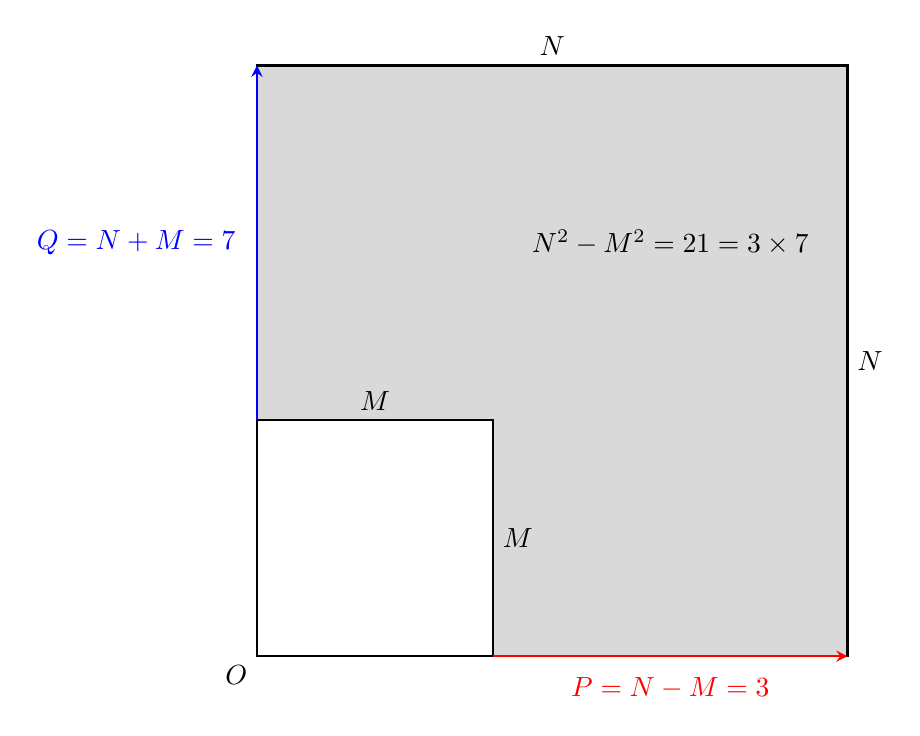
\begin{tikzpicture}[scale=1.5,>=stealth]
% Outer square of side N=5 and inner square of side M=2
\draw[thick] (0,0) rectangle (5,5);
\draw[thick] (0,0) rectangle (2,2);
\draw[dashed,thick] (2,2) rectangle (5,5);
% L-shaped region
\fill[gray!30] (2,0) rectangle (5,5);
\fill[gray!30] (0,2) rectangle (2,5);
\draw[thick] (0,0) rectangle (5,5);
\draw[thick] (0,0) rectangle (2,2);
\node[below left] at (0,0) {$O$};
\node[above] at (2.5,5) {$N$};
\node[above] at (1,2) {$M$};
\node[right] at (5,2.5) {$N$};
\node[right] at (2,1) {$M$};
% P = N - M and Q = N + M
\draw[red,thick,->] (2,0) -- (5,0);
\node[below,red] at (3.5,-0.1) {$P=N-M=3$};
\draw[blue,thick,->] (0,2) -- (0,5);
\node[left,blue] at (-0.1,3.5) {$Q=N+M=7$};
\node at (3.5,3.5) {$N^2-M^2=21=3\times 7$};
\end{tikzpicture}
\caption{The geometric construction for $N=5$, $M=2$: The L-shaped region has area $N^2 - M^2 = 25 - 4 = 21 = 3 \times 7$, a semiprime. The factors $P=3$ and $Q=7$ are both prime and sum to $2N=10$, providing the Goldbach partition $10 = 3 + 7$.}
\label{fig:geometric}
\end{figure}
\subsection{Reformulation as a Centered Set Intersection Problem}\label{subsec:setintersection}
Let
\[
A_N=\{1,2,\ldots,N-3\}
\]
be the admissible range for $M$. For each $N \geq 4$, define two centered subsets of $A_N$:
\begin{itemize}
\item \textbf{Lower-prime candidate set:} $C_N = \{M\in A_N \mid N-M \text{ is prime}\}$.
\item \textbf{Upper-prime candidate set:} $D_N = \{M\in A_N \mid N+M \text{ is prime}\}$.
\end{itemize}
Both centered sets lie in a single parity class. Indeed, if $N-M$ or $N+M$ is an odd prime, then $M$ has parity opposite to $N$. Thus
\[
C_N,D_N\subseteq B_N:=\{M\in A_N\mid M\not\equiv N\pmod 2\}.
\]
\begin{Proposition}[Centered intersection criterion]\label{prop:intersection}
The distinct-prime Goldbach conjecture holds for the even integer $2N$ ($N \geq 4$) if and only if $C_N \cap D_N \neq \emptyset$.
\end{Proposition}
\begin{proof}
\textbf{($\Rightarrow$)} Suppose $2N = p + q$ with distinct primes $p < q$. Set $M = (q-p)/2$. As in the proof of Theorem~\ref{thm:geometric}, $M \in A_N$, $p=N-M$, and $q=N+M$. Hence $M\in C_N\cap D_N$.

\textbf{($\Leftarrow$)} Suppose $M \in C_N \cap D_N$. Then $N-M$ is prime by the definition of $C_N$, and $N+M$ is prime by the definition of $D_N$. Their sum is $2N$, and they are distinct because $M\geq 1$.
\end{proof}

\subsection{The Case $M=0$}\label{subsec:M-zero}
For $N\geq 3$ let $\overline{A}_N=\{0,1,\ldots,N-3\}$, let $\overline{C}_N$ and $\overline{D}_N$ be the sets of $M\in\overline{A}_N$ with $N-M$ prime and $N+M$ prime respectively, let $\overline{E}_N$ be the set of $M\in\overline{A}_N$ with $M=(Q-P)/2$ for primes $2<P\leq N\leq Q<2N$, and let $\overline{R}(2N)=|\overline{C}_N\cap\overline{D}_N|$.
\begin{Proposition}[The diagonal]\label{prop:M-zero}
For every integer $N\geq 3$, $0\in\overline{C}_N\cap\overline{D}_N$ if and only if $N$ is prime; $0\in\overline{E}_N$ if and only if $N$ is an odd prime; and $\overline{R}(2N)=R(2N)+\mathbf 1_{N\text{ prime}}$. For $N\geq 4$, $\overline{R}(2N)\geq 1$ if and only if $2N$ is a sum of two primes.
\end{Proposition}
\begin{proof}
The element $M=0$ gives $N-0=N+0=N$, so it lies in $\overline{C}_N\cap\overline{D}_N$ exactly when $N$ is prime. If $M=0$ in $\overline{E}_N$, then $P=Q$, and $P\leq N\leq Q$ gives $P=Q=N$; conversely an odd prime $N$ gives $P=Q=N$ and $N<2N$. The elements $M\geq 1$ of $\overline{C}_N\cap\overline{D}_N$ are those of $C_N\cap D_N$, which gives the formula for $\overline{R}(2N)$. The last statement follows from Proposition~\ref{prop:intersection} and the fact that $2N=N+N$ with $N$ prime is the only partition into equal primes.
\end{proof}

\subsection{The Half-Difference Diagnostic Set}\label{subsec:diagnostic}
It is useful computationally to compare the centered sets with a set of half-differences arising from straddling prime pairs. Define
\[
E_N =
\left\{
\frac{Q-P}{2}\in A_N \;\middle|\; 2<P<N<Q<2N,\; P,Q \text{ prime}
\right\}.
\]
The restriction $\frac{Q-P}{2}\in A_N$ is part of the definition, so every listed element of $E_N$ lies in $\{1,\ldots,N-3\}$. The set $E_N$ measures the availability of prime-pair differences near $N$, while $D_N$ measures primality of the centered upper endpoint $N+M$. The proof target remains the centered intersection $C_N\cap D_N$.

\begin{Lemma}\label{lem:CD-in-E}
For every $N\geq 4$,
\[
C_N\cap D_N\subseteq E_N.
\]
Consequently, $C_N\cap E_N\cap D_N=C_N\cap D_N$.
\end{Lemma}
\begin{proof}
Let $M\in C_N\cap D_N$, and set $P=N-M$ and $Q=N+M$. Both are prime, and $M\in A_N$ gives $P\geq 3>2$, $P<N<Q$ and $Q\leq 2N-3<2N$. Since $M=\frac{Q-P}{2}\in A_N$, we get $M\in E_N$. The second statement follows by intersecting both sides with $C_N$.
\end{proof}

\begin{Lemma}[Gap obstruction]\label{lem:gap}
Let $N\geq 4$, let $p^-$ be the largest prime below $N$, and let $p^+$ be the smallest prime above $N$. If $M\in E_N$, then $2M\geq p^+-p^-$. Hence every $M\in A_N$ with $M<(p^+-p^-)/2$ lies in $A_N\setminus E_N$.
\end{Lemma}
\begin{proof}
If $M=(Q-P)/2$ with primes $P<N<Q$, then $P\leq p^-$ and $Q\geq p^+$, so $2M=Q-P\geq p^+-p^-$.
\end{proof}

\begin{Lemma}[Upper gap obstruction]\label{lem:gap-top}
Let $N\geq 4$, and let $q$ be the largest prime below $2N$. If $M\in E_N$, then $2M\leq q-3$. Hence every $M\in A_N$ with $M>(q-3)/2$ lies in $A_N\setminus E_N$; if $q\leq 2N-3$, there are $(2N-3-q)/2$ such values.
\end{Lemma}
\begin{proof}
If $M=(Q-P)/2$ with primes $2<P$ and $Q<2N$, then $P\geq 3$ and $Q\leq q$, so $2M\leq q-3$. The values $M\in A_N$ with $M>(q-3)/2$ are $M=(q-3)/2+1,\ldots,N-3$, and there are $N-3-(q-3)/2=(2N-3-q)/2$ of them.
\end{proof}

\subsection{Nearby Even Numbers Represented by $E_N$}\label{subsec:nearby-even}
Each element of $E_N$ arises from a Goldbach partition of a nearby even number. If $M\in E_N$, then there exist odd primes $P,Q$ such that
\[
2<P<N<Q<2N,\qquad M=\frac{Q-P}{2},
\]
and the even number
\[
S=P+Q
\]
has a Goldbach partition with half-difference $M$. Conversely, any Goldbach partition $S=P+Q$ satisfying these inequalities and $\frac{Q-P}{2}\in A_N$ contributes its half-difference to $E_N$.

The possible sums $S$ lie in the even part of the interval
\[
N+4\leq S\leq 3N-2,
\]
with endpoint adjustments forced by parity and by the primality of $P$ and $Q$. If one excludes the endpoint possibility $Q=2N-1$, the upper endpoint becomes $3N-4$ when $N$ is even. The centered Goldbach problem for $2N$ is the special case $S=2N$, where the partition has the form
\[
2N=(N-M)+(N+M).
\]

\subsection{Lower and Upper Primes}\label{subsec:upper-prime-count}
Let
\[
L_N=\{P\mid 3\leq P<N,\; P \text{ prime}\},\qquad
a_N=|L_N|=\pi(N-1)-1,
\]
and let
\[
U_N=\{Q\mid N<Q\leq 2N-3,\; Q \text{ prime}\}
=\{Q_1>Q_2>\cdots>Q_r\}.
\]
If $2N-3$ is prime, then $2N=3+(2N-3)$ is already a centered Goldbach partition with $M=N-3$. For estimates of $r$, the only possible prime counted by $\pi(2N)-\pi(N)$ but not by $\pi(2N-3)-\pi(N)$ is $2N-1$. Hence
\[
\pi(2N)-\pi(N)-1\leq r\leq \pi(2N)-\pi(N).
\]
Proposition~\ref{prop:rs-dyadic} therefore gives, for $N\geq 41/2$,
\[
\frac{3N}{5\log N}-1<r<\frac{7N}{5\log N}.
\]
For $P\in L_N$ and $Q\in U_N$ we have $3\leq P<N<Q\leq 2N-3$, so $1\leq (Q-P)/2\leq N-3$; hence $(Q-P)/2\in E_N$ for every pair $(P,Q)\in L_N\times U_N$. For $d>0$ define
\[
\rho_L(d)=\#\{(P,P')\in L_N^2\mid P'-P=d\},
\qquad
\rho_U(d)=\#\{(i,j)\mid i<j,\; Q_i-Q_j=d\},
\]
and the additive energy
\[
\mathcal C_N
=
\sum_{d>0}\rho_L(d)\rho_U(d),
\]
which counts the quadruples $(P,P',Q_i,Q_j)$ with $P,P'\in L_N$, $i<j$ and $P'-P=Q_i-Q_j$.

\subsection{A Linear Lower Bound for the Half-Difference Set}\label{subsec:linear}
The additive energy $\mathcal C_N$ of Section~\ref{subsec:upper-prime-count} controls $|E_N|$ from below, through the Cauchy--Schwarz inequality. We use the following explicit sieve bound of Siebert, stated in~\cite{siebert1976montgomery} for primes $p$ with $ap+b$ prime, $2\mid ab$; we take $a=1$ and $b=h$.
\begin{Proposition}[{\cite{siebert1976montgomery}}]\label{prop:siebert}
Let
\[
\omega=\prod_{p>2}\left(1-\frac{1}{(p-1)^2}\right),\qquad
\kappa(h)=\prod_{\substack{p\mid h\\ p>2}}\frac{p-1}{p-2}.
\]
For every real number $x>1$ and every even integer $h\neq 0$,
\[
\#\{p\leq x \mid p \text{ and } p+h \text{ are prime}\}\leq 16\,\omega\,\kappa(h)\,\frac{x}{\log^2 x}.
\]
\end{Proposition}
For $M\in A_N$ define
\[
\nu_N(M)=\#\{(P,Q)\in L_N\times U_N\mid Q-P=2M\}.
\]
Every pair $(P,Q)\in L_N\times U_N$ gives $(Q-P)/2\in E_N$, as shown in Section~\ref{subsec:upper-prime-count}. Hence $\nu_N$ vanishes outside $E_N$, and
\[
\sum_{M\in E_N}\nu_N(M)=a_N\,r.
\]
\begin{Lemma}[Energy identity]\label{lem:energy}
For every $N\geq 4$,
\[
\sum_{M\in A_N}\nu_N(M)^2=a_N\,r+2\,\mathcal C_N.
\]
\end{Lemma}
\begin{proof}
The left-hand side counts the quadruples $(P,Q,P',Q')\in L_N\times U_N\times L_N\times U_N$ with $Q-P=Q'-P'$, that is, with $P'-P=Q'-Q=:h$. The value $h=0$ gives $P=P'$ and $Q=Q'$, hence $a_N r$ quadruples. For $h>0$ the number of quadruples is $\rho_L(h)\rho_U(h)$, and exchanging $(P,Q)$ with $(P',Q')$ maps the quadruples with difference $h$ bijectively onto those with difference $-h$.
\end{proof}
\begin{Lemma}[Energy bound]\label{lem:energy-bound}
Let
\[
G=\prod_{p>2}\left(1+\frac{2p-3}{p(p-2)^2}\right).
\]
For every $N\geq 4$,
\[
\mathcal C_N\leq 256\,\omega^2 G\,\frac{N^3}{\log^4 N}.
\]
Moreover, $\omega<0.6614$ and $G<2.658$.
\end{Lemma}
\begin{proof}
All primes in $L_N\cup U_N$ are odd, so $\rho_L(h)=0$ unless $h$ is even with $2\leq h\leq N-4$. For such $h$, Proposition~\ref{prop:siebert} with $x=N$ and with $x=2N$ gives
\[
\rho_L(h)\leq 16\,\omega\,\kappa(h)\frac{N}{\log^2 N},\qquad
\rho_U(h)\leq 16\,\omega\,\kappa(h)\frac{2N}{\log^2 (2N)}\leq 32\,\omega\,\kappa(h)\frac{N}{\log^2 N},
\]
since every pair counted by $\rho_U(h)$ consists of primes $Q<Q+h\leq 2N$. Hence
\[
\mathcal C_N\leq 512\,\omega^2\frac{N^2}{\log^4 N}\sum_{1\leq k\leq N/2}\kappa(2k)^2.
\]
Since $\kappa$ depends only on the odd prime divisors, $\kappa(2k)=\kappa(k)$. The function $\kappa^2$ satisfies $\kappa(k)^2=\sum_{d\mid k}g(d)$, where $g$ is the multiplicative function supported on odd squarefree integers with
\[
g(p)=\left(\frac{p-1}{p-2}\right)^2-1=\frac{2p-3}{(p-2)^2}\qquad(p>2).
\]
Since $g\geq 0$, for every $K\geq 1$
\[
\sum_{k\leq K}\kappa(k)^2=\sum_{d\leq K}g(d)\left\lfloor\frac{K}{d}\right\rfloor\leq K\sum_{d\geq 1}\frac{g(d)}{d}=K\,G.
\]
Taking $K=N/2$ gives the bound for $\mathcal C_N$.

Every factor of $\omega$ lies in $(0,1)$, so $\omega$ is at most the product of its factors with $3\leq p\leq 97$, which is less than $0.66138$. For $G$, the product of its factors with $3\leq p\leq 97$ is less than $2.63013$. For $p\geq 101$ we have $\frac{2p-3}{p(p-2)^2}<\frac{2}{(p-2)^2}$ and $p-2$ is odd, so, using $\log(1+y)\leq y$,
\begin{align*}
\log\prod_{p\geq 101}\left(1+\frac{2p-3}{p(p-2)^2}\right)&<2\sum_{\substack{m\geq 99\\ m \text{ odd}}}\frac{1}{m^2}\leq 2\left(\frac{1}{99^2}+\frac{1}{2}\int_{99}^{\infty}\frac{dt}{t^2}\right)\\
&=2\left(\frac{1}{9801}+\frac{1}{198}\right)<0.01031.
\end{align*}
Hence $G<2.63013\,e^{0.01031}<2.658$.
\end{proof}
\begin{Theorem}[Linear lower bound]\label{thm:linear}
For every integer $N\geq 3275$,
\[
|E_N|>\frac{N}{760}.
\]
\end{Theorem}
\begin{proof}
Write $L=\log N$ and $\lambda=\log 2$. By the Cauchy--Schwarz inequality and Lemma~\ref{lem:energy},
\[
(a_N r)^2=\Bigl(\sum_{M\in E_N}\nu_N(M)\Bigr)^2\leq |E_N|\sum_{M\in A_N}\nu_N(M)^2=|E_N|\,(a_N r+2\mathcal C_N).
\]
\emph{Lower bound for $a_N r$.} By Proposition~\ref{prop:rs-pi} with $x=N-1\geq 17$, $a_N=\pi(N-1)-1>\frac{N-1}{L}-1$, so
\[
a_N>\frac{N}{L}\,\mathcal A(N),\qquad \mathcal A(N)=1-\frac{1+L}{N}.
\]
As shown in Section~\ref{subsec:upper-prime-count}, $r\geq \pi(2N)-\pi(N)-1$. Proposition~\ref{prop:dusart-upper}\emph{(1)} with $x=2N\geq 599$ and Proposition~\ref{prop:dusart-upper}\emph{(2)} with $x=N$ give
\[
r\geq \frac{2N}{L+\lambda}\left(1+\frac{1}{L+\lambda}\right)-\frac{N}{L}\left(1+\frac{1.2762}{L}\right)-1=\frac{N}{L}\,\mathcal B(N),
\]
where, using $\frac{2L}{L+\lambda}=2-\frac{2\lambda}{L+\lambda}$,
\[
\mathcal B(N)=1-\frac{2\lambda}{L+\lambda}+\frac{2L}{(L+\lambda)^2}-\frac{1.2762}{L}-\frac{L}{N}.
\]
Both $\mathcal A$ and $\mathcal B$ are increasing in $N$ for $N\geq 3275$. For $\mathcal A$ this holds because $(1+\log x)/x$ is decreasing for $x>1$. For $\mathcal B$, the term $-L/N$ is increasing for $N>e$, and the derivative with respect to $L$ of the remaining terms is
\begin{align*}
\frac{2\lambda(\lambda+1)-(2-2\lambda)L}{(L+\lambda)^3}+\frac{1.2762}{L^2}&>-\frac{(2-2\lambda)L}{L^3}+\frac{1.2762}{L^2}\\
&=\frac{1.2762-(2-2\lambda)}{L^2}>0,
\end{align*}
since $2-2\lambda<0.614$; here the first numerator is negative for $L\geq\log 3275$. At $N=3275$, $\mathcal A>0.99722$ and $\mathcal B>0.89174$. Hence, for every $N\geq 3275$,
\[
a_N r>\alpha\,\frac{N^2}{L^2},\qquad \alpha=0.8892.
\]
\emph{Conclusion.} The function $t\mapsto t^2/(t+K)$ is increasing for $t>0$, and decreasing in $K>0$. With $X=\alpha N^2/L^2$ and, by Lemma~\ref{lem:energy-bound}, $2\mathcal C_N\leq \overline K=\beta N^3/L^4$, where $\beta=512\cdot 0.6614^2\cdot 2.658<595.33$, we obtain
\[
|E_N|\geq\frac{(a_N r)^2}{a_N r+2\mathcal C_N}>\frac{X^2}{X+\overline K}=\frac{\alpha^2 N}{\beta\,(1+\delta_N)},\qquad \delta_N=\frac{X}{\overline K}=\frac{\alpha L^2}{\beta N}.
\]
The function $t\mapsto \log^2 t/t$ is decreasing for $t>e^2$, so $\delta_N\leq \delta_{3275}<3\cdot 10^{-5}$. Therefore
\[
|E_N|>\frac{0.8892^2}{595.33\cdot 1.00003}\,N>0.001328\,N>\frac{N}{760}.
\]
\end{proof}
By definition, $M\in E_N$ if and only if there is a prime $p$ with $\max\{2,N-2M\}<p<N$ such that $p+2M$ is a prime smaller than $2N$. For a fixed shift $2k$, the number of primes $p\leq y$ with $p+2k$ prime is conjectured by Hardy and Littlewood to be asymptotic to $2\omega\kappa(2k)\,y/\log^2 y$, and this asymptotic is known for almost all shifts. Wolke~\cite{wolke1989primzahl} proved it for almost all $k\leq x$ and all $y\in[2x,x^{8/5-\varepsilon}]$, improving earlier results of Lavrik~\cite{lavrik1961number}. Mikawa~\cite{mikawa1991prime} extended the range of $y$ substantially: for every $\varepsilon,A,B>0$ and all sufficiently large $x$, the asymptotic
\[
\Psi(y,2k)=\mathfrak S(2k)(y-2k)+O\bigl(y/(\log y)^B\bigr)
\]
holds for all but $O(x(\log x)^{-A})$ integers $k\leq x$, whenever $2x\leq y\leq x^{3-\varepsilon}$. (Here $\Psi(y,2k)=\sum_{2k<n\leq y}\Lambda(n)\Lambda(n-2k)$.) Perelli and Pintz~\cite{perelli1992exceptional} proved a version for all but $O(H(\log N)^{-B})$ shifts $2k$ with $k$ in intervals of length $H$, in the range $N^{1/2+\varepsilon}\leq H\leq N/4$. More recently, Matom\"aki, Radziwi{\l}{\l} and Tao~\cite{matomaki2019correlations} obtained a further improvement on the lower end of the difference range: the Hardy--Littlewood asymptotic for $\sum_{X<n\leq 2X}\Lambda(n)\Lambda(n+h)$ holds for all but $O(H(\log X)^{-A})$ values of $h$ with $|h-h_0|\leq H$, whenever $X^{8/33+\varepsilon}\leq H\leq X^{1-\varepsilon}$ and $0\leq h_0\leq X^{1-\varepsilon}$. Their argument also covers mixed correlations involving the divisor functions $d_k$ and yields an averaged binary Goldbach asymptotic in short intervals. These results are stated with unspecified constants; the present paper relies only on Mikawa's theorem (stated as Proposition~\ref{prop:mikawa} below) in the restricted range $2x\leq y\leq 4x$.

Let
\[
\Psi(y,2k)=\sum_{2k<n\leq y}\Lambda(n)\Lambda(n-2k),
\]
where $\Lambda$ is the von Mangoldt function, and let $\mathfrak S(2k)=2\omega\kappa(2k)$ be the singular series, so that $\mathfrak S(2k)\geq 2\omega$.
\begin{Proposition}[{\cite{mikawa1991prime}}]\label{prop:mikawa}
Let $\varepsilon,A,B>0$. For all sufficiently large $x$ and every $y$ with $2x\leq y\leq x^{3-\varepsilon}$, all but $O(x(\log x)^{-A})$ integers $k$ with $1\leq k\leq x$ satisfy
\[
\Psi(y,2k)=\mathfrak S(2k)(y-2k)+O\!\left(\frac{y}{(\log y)^{B}}\right),
\]
where the implied constants depend only on $\varepsilon$, $A$ and $B$.
\end{Proposition}
We use Proposition~\ref{prop:mikawa} only for $2x\leq y\leq 4x$.
\begin{Proposition}[Almost all half-differences]\label{prop:almost-all}
For every $D>0$,
\[
|A_N\setminus E_N|\ll_D\frac{N}{(\log N)^D}.
\]
In particular, $|E_N|=N-o(N)$.
\end{Proposition}
\begin{proof}
Write $L=\log N$ and $a=\lceil N/L^D\rceil$, and apply Proposition~\ref{prop:mikawa} with $\varepsilon=1/2$, $A=D$ and $B=D+1$. The terms of $\Psi(y,2k)$ with $y\leq 2N$ in which $n$ or $n-2k$ is a prime power $p^j$ with $j\geq 2$ contribute $O(\sqrt N L^3)$, since there are $O(\sqrt N L)$ such prime powers up to $2N$ and each term is at most $L^2+O(L)$.

\emph{The range $a<k\leq N/2$.} Take $x=N/2$ and the two values $y_1=N$ and $y_2=N+2a$, which satisfy $2x\leq y_1<y_2\leq 4x$. Outside a set of $O(NL^{-D})$ integers $k\leq x$, Proposition~\ref{prop:mikawa} applies to both values, and
\begin{align*}
\Psi(y_2,2k)-\Psi(y_1,2k)&=\sum_{N<n\leq N+2a}\Lambda(n)\Lambda(n-2k)\\
&=2a\,\mathfrak S(2k)+O\!\left(\frac{N}{L^{D+1}}\right)\geq 4\omega a-O\!\left(\frac{N}{L^{D+1}}\right),
\end{align*}
which exceeds the prime-power contribution $O(\sqrt N L^3)$ for large $N$. Hence there is an integer $n$ with $N<n\leq N+2a$ such that $Q=n$ and $P=n-2k$ are both prime. Then $N<Q<2N$, and $P\leq N+2a-2k<N$ because $k>a$; moreover $P$ is odd, because $Q$ is odd and $2k$ is even, so $P>2$. Thus $k\in E_N$.

\emph{The range $N/2<k\leq N-3-a$.} Take $x=N-1$ and $y=2N-1$, so that $2x\leq y\leq 4x$. Outside a set of $O(NL^{-D})$ integers $k\leq x$,
\[
\Psi(2N-1,2k)=\mathfrak S(2k)(2N-1-2k)+O\!\left(\frac{N}{L^{D+1}}\right)\geq 2\omega(2a+5)-O\!\left(\frac{N}{L^{D+1}}\right),
\]
which exceeds $O(\sqrt N L^3)$ for large $N$. Hence there is an integer $n$ with $2k<n\leq 2N-1$ such that $Q=n$ and $P=n-2k$ are both prime. Then $N<2k<Q<2N$ and $P\leq 2N-1-2k<N$, and $P>2$ as before. Thus $k\in E_N$.

\emph{Conclusion.} The remaining integers $k\in A_N$ satisfy $k\leq a$ or $k>N-3-a$, and there are at most $2a$ of them. Hence $|A_N\setminus E_N|\leq 2a+O(NL^{-D})\ll_D N/L^D$.
\end{proof}

\begin{Corollary}[Goldbach partitions up to a difference of two primes]\label{cor:goldbach-diff}
For every $D>0$,
\[
|C_N\cap E_N|=\pi(N-1)-1+O_D\!\left(\frac{N}{(\log N)^D}\right).
\]
Equivalently, for all but $O_D(N/(\log N)^D)$ primes $P$ with $3\leq P<N$ there are primes $P'$ and $Q'$ with $2<P'<N<Q'<2N$ and
\[
Q'=(2N-P)+(P'-P).
\]
In particular, $C_N\cap E_N\neq\emptyset$ for all sufficiently large $N$. The case $P'=P$ is a distinct-prime Goldbach partition $2N=P+Q'$.
\end{Corollary}
\begin{proof}
The map $M\mapsto N-M$ is a bijection from $C_N$ onto the set of primes $P$ with $3\leq P\leq N-1$, so $|C_N|=\pi(N-1)-1$. Since $|C_N|-|A_N\setminus E_N|\leq|C_N\cap E_N|\leq|C_N|$, Proposition~\ref{prop:almost-all} gives the first statement. For a prime $3\leq P<N$, the value $M=N-P$ lies in $A_N$, and $M\in E_N$ if and only if $2(N-P)=Q'-P'$ for primes $2<P'<N<Q'<2N$, that is, $Q'=(2N-P)+(P'-P)$. Finally, $\pi(N-1)-1>(N-1)/\log N-1$ by Proposition~\ref{prop:rs-pi}, which exceeds the error term for large $N$.
\end{proof}
Proposition~\ref{prop:almost-all} is deduced from Proposition~\ref{prop:mikawa} and gives no explicit value of $N$ from which a stated bound holds. Theorem~\ref{thm:linear} gives the explicit bound $|E_N|>N/760$ for every $N\geq 3275$.

\subsection{A Positive Proportion of Centered Partitions}\label{subsec:positive-proportion}
The same energy method applies to the centered count
\[
R(2N)=|C_N\cap D_N|=\#\{p\mid 3\leq p<N,\; p \text{ and } 2N-p \text{ prime}\}.
\]
\begin{Theorem}[Positive proportion]\label{thm:positive-proportion}
For every real number $X\geq 10^6$,
\[
\#\{N\in\mathbb Z\mid 4\leq N\leq X,\; R(2N)\geq 1\}>\frac{X}{2382}.
\]
\end{Theorem}
\begin{proof}
Write $L=\log X$ and $s=X/L$, and let $S$ be the set of odd primes not exceeding $2X$. Let
\[
T=\sum_{4\leq N\leq X}R(2N),\qquad V=\sum_{4\leq N\leq X}R(2N)^2.
\]
By the Cauchy--Schwarz inequality, the number of $N$ with $R(2N)\geq 1$ is at least $T^2/V$.

\emph{Lower bound for $T$.} Every pair of odd primes $p<q\leq X$ gives $N=(p+q)/2$ with $4\leq N<X$ and $M=N-p\in C_N\cap D_N$, and distinct pairs give distinct pairs $(N,p)$ counted by $R(2N)$. Hence, by Proposition~\ref{prop:rs-pi},
\[
T\geq\binom{\pi(X)-1}{2}>\frac{(s-2)^2}{2}.
\]
\emph{Upper bound for $V$.} The square $R(2N)^2$ counts pairs of representations $2N=p+q=p'+q'$ with $3\leq p<N<q\leq 2N-3$ and $3\leq p'<N<q'\leq 2N-3$. For $N\leq X$ the primes $p,p'$ are odd and at most $X$, and the primes $q,q'$ are odd and at most $2X$. Let $S_X$ and $S_{2X}$ be the sets of odd primes not exceeding $X$ and $2X$. Then $V$ is at most the number of quadruples $(p,q,p',q')\in S_X\times S_{2X}\times S_X\times S_{2X}$ with $p+q=p'+q'$, that is, with $p'-p=q-q'=:h$. For $Y\in\{X,2X\}$ let $\rho_Y(h)=\#\{(a,b)\in S_Y^2\mid b-a=h\}$. The number of quadruples is $\sum_h\rho_X(h)\rho_{2X}(h)$, where $\rho_Y(-h)=\rho_Y(h)$ and $\rho_Y(h)=0$ for odd $h$. The value $h=0$ contributes $|S_X||S_{2X}|\leq\pi(X)\pi(2X)$. For even $h$ with $2\leq h\leq X$, Proposition~\ref{prop:siebert} with $x=X$ and with $x=2X$ gives
\[
\rho_X(h)\leq 16\,\omega\,\kappa(h)\frac{X}{L^2},\qquad
\rho_{2X}(h)\leq 16\,\omega\,\kappa(h)\frac{2X}{\log^2(2X)}\leq 32\,\omega\,\kappa(h)\frac{X}{L^2},
\]
and $\rho_X(h)=0$ for $h>X$. As in the proof of Lemma~\ref{lem:energy-bound}, $\sum_{2\leq h\leq X,\,h \text{ even}}\kappa(h)^2\leq XG/2$. Hence
\[
V\leq \pi(X)\pi(2X)+2\cdot 512\,\omega^2\frac{X^2}{L^4}\,\frac{XG}{2}=\pi(X)\pi(2X)+K\frac{X^3}{L^4},\qquad K=512\,\omega^2 G.
\]
By Proposition~\ref{prop:dusart-upper}\emph{(2)}, $\pi(X)\leq \frac{X}{L}\bigl(1+\frac{1.2762}{L}\bigr)$, and since $y\mapsto \frac1y\bigl(1+\frac{1.2762}{y}\bigr)$ is decreasing, $\pi(2X)\leq \frac{2X}{L}\bigl(1+\frac{1.2762}{L}\bigr)$.

\emph{Conclusion.} Since $X^3/L^4=s^4/X$,
\[
\frac{T^2}{V}>\frac{(s-2)^4/4}{2s^2\bigl(1+\frac{1.2762}{L}\bigr)^2+K s^4/X}=\frac{X\,(1-2/s)^4}{4\bigl(K+e(X)\bigr)},
\]
where $e(X)=\frac{2L^2}{X}\bigl(1+\frac{1.2762}{L}\bigr)^2$.
For $X\geq 10^6$, $s$ is increasing and $e(X)$ is decreasing, so $(1-2/s)^4>0.99988$ and $e(X)<0.00046$. By Lemma~\ref{lem:energy-bound}, $K<512\cdot 0.6614^2\cdot 2.658<595.33$. Therefore
\[
\frac{T^2}{V}>\frac{0.99988}{4\cdot 595.33046}\,X>\frac{X}{2382}.
\]
\end{proof}
Montgomery and Vaughan~\cite{montgomery1975exceptional} proved that, for some $\delta>0$ and all sufficiently large $X$, at most $X^{1-\delta}$ even integers $n\leq X$ are not sums of two primes. The survey~\cite{bhowmik2026exceptional} records that Chudakov, van der Corput and Estermann proved $E(X)\ll_A X(\log X)^{-A}$ for every $A>0$, by a proof that uses the Siegel--Walfisz theorem, whose implied constant is ineffective (its Theorem~4.3 and equation~(4.1)); that the exponent $\delta$ of Montgomery and Vaughan is effectively computable (Section~1.1); and that Pintz proved $E(X)<X^{0.72}$ for all sufficiently large $X$, with an ineffective constant (its Proposition~6.4). Here $E(X)$ is the number of even integers $n$ with $4\leq n\leq X$ that are not sums of two primes. Recent results on this exceptional set and on prime pairs are in Section~\ref{subsec:recent}. Theorem~\ref{thm:positive-proportion} is weaker in its conclusion than the bounds there, but it is explicit and holds for every $X\geq 10^6$. By Proposition~\ref{prop:verified}, its conclusion is trivial for $X\leq 2\cdot 10^{18}$.

\subsection{Recent Results on the Exceptional Set and on Prime Pairs}\label{subsec:recent}
Let $G(n)$ be the number of ordered pairs $(p_1,p_2)$ of primes with $2<p_1,p_2<n$ and $p_1+p_2=n$, and let $E(X)$ be the number of even integers $n$ with $4\leq n\leq X$ that are not sums of two primes, where the two primes may be equal. Let $H_\theta$ be the assertion that every nontrivial zero $\rho$ of the $L$-function of every primitive Dirichlet character, including $\zeta(s)$, satisfies $\operatorname{Re}\rho\leq\theta$. The generalized Riemann hypothesis for Dirichlet $L$-functions is $H_{1/2}$. A Lean proof of the Riemann hypothesis and of its generalization to Dirichlet $L$-functions was released by Alp\"oge on 20 November 2026~\cite{alpoge2026}, and the Lean FRO and the Mathlib Initiative certified the statement and the proof of the Riemann hypothesis~\cite{leanfro2026}.

Pintz and Alth\"ofer~\cite{pintz2026exceptional} prove, in an arXiv preprint, that $H_{\theta_0}$ for a fixed $1/2\leq\theta_0<1$ implies $E(X)\ll_{\theta_0,\varepsilon}X^{7/12+\varepsilon}$ for every $\varepsilon>0$ (their Theorem~1), and that $H_\theta$ for a fixed $1/2\leq\theta\leq 2/3$ implies $E(X)\ll_{\theta,\varepsilon}X^{g(\theta)+\varepsilon}$ for every $\varepsilon>0$ (their Theorem~3), where
\[
g(\theta)=\frac{\theta(5-4\theta)}{2(2-\theta)}=2\theta-\frac32+\frac{3(1-\theta)}{2-\theta}.
\]
The function $g$ is strictly increasing on $[1/2,2/3]$, with $g(1/2)=1/2$, $g(5/8)=25/44$ and $g(2/3)=7/12$. Since $7/12-25/44=1/66$, $H_{5/8}$ gives an exponent smaller than $7/12$ by $1/66$. Bhowmik and Grimmelt~\cite{bhowmik2026exceptional} state, as Theorem~3.1 of their survey, the following bound of Hardy and Littlewood: if every zero of every Dirichlet $L$-function has real part at most $\Theta<3/4$, then $E(X)\ll_\varepsilon X^{2\Theta-1/2+\varepsilon}$ for every $\varepsilon>0$. For $\Theta=1/2$ the exponent is $1/2$.

\begin{Proposition}[Consequence of $H_{1/2}$]\label{prop:E-half}
By Theorem~3 of~\cite{pintz2026exceptional} with $\theta=1/2$ and by the generalized Riemann hypothesis~\cite{alpoge2026}, $E(X)\ll_\varepsilon X^{1/2+\varepsilon}$ for every $\varepsilon>0$.
\end{Proposition}

The next proposition relates $E(X)$ to the exceptional set for sums of two distinct primes.
\begin{Proposition}[Distinct primes and the exceptional set]\label{prop:E-distinct}
Let $E'(X)$ be the number of even integers $n$ with $4\leq n\leq X$ that are not sums of two distinct primes. If $N$ is not prime, then $2N$ is a sum of two primes if and only if it is a sum of two distinct primes. Consequently $E(X)\leq E'(X)\leq E(X)+\pi(X/2)$.
\end{Proposition}
\begin{proof}
If $2N=p+q$ with $p=q$, then $N=p$ is prime. Hence, for $N$ not prime, every representation of $2N$ as a sum of two primes has distinct primes. A sum of two distinct primes is a sum of two primes, which gives $E(X)\leq E'(X)$. An even integer that is a sum of two primes but not of two distinct primes equals $2p$ with $p$ prime and $2p\leq X$, and there are at most $\pi(X/2)$ of these.
\end{proof}

\begin{Corollary}[Many centered partitions under $H_{1/2}$]\label{cor:cnt-GRH}
For every $\varepsilon>0$ there is a constant $C_\varepsilon$ such that, for every sufficiently large integer $X$,
\[
\#\{N\in\mathbb Z\mid 4\leq N\leq X,\; R(2N)\geq 1\}\ \geq\ X-3-\pi(X)-C_\varepsilon X^{1/2+\varepsilon}.
\]
\end{Corollary}
\begin{proof}
Let $4\leq N\leq X$ with $R(2N)=0$. By Proposition~\ref{prop:intersection}, $2N$ is not a sum of two distinct primes, so $2N$ is counted by $E'(2X)$. By Proposition~\ref{prop:E-distinct} with $X$ replaced by $2X$, $E'(2X)\leq E(2X)+\pi(X)$, and by Proposition~\ref{prop:E-half}, $E(2X)\leq C(2X)^{1/2+\varepsilon}$ for all sufficiently large $X$. There are $X-3$ integers $N$ with $4\leq N\leq X$.
\end{proof}

Johnston and Trudgian~\cite{johnston2026linnik} use the bound of Lichtman~\cite{lichtman2023goldbach} for prime pairs. For every $\varepsilon>0$ and every sufficiently large even $n$,
\begin{equation}\label{eq:lichtman}
G(n)\leq (C^*+\varepsilon)\,\omega\,\kappa(n)\frac{n}{\log^2 n},\qquad C^*=6.7814,
\end{equation}
with $\omega$ and $\kappa$ as in Proposition~\ref{prop:siebert}; under the Elliott--Halberstam conjecture the same bound holds with $C^*=4$~\cite{johnston2026linnik}.

\begin{Proposition}[Centered partitions and prime pairs]\label{prop:R-upper}
For every integer $N\geq 4$, $2R(2N)\leq G(2N)$. Consequently, for every $\varepsilon>0$ and every sufficiently large $N$,
\[
R(2N)\leq\left(\frac{C^*}{2}+\varepsilon\right)\omega\,\kappa(2N)\frac{2N}{\log^2(2N)}
\]
with $C^*$ as in~\eqref{eq:lichtman}.
\end{Proposition}
\begin{proof}
Each $M\in C_N\cap D_N$ gives the two ordered pairs $(N-M,N+M)$ and $(N+M,N-M)$ of primes in $(2,2N)$ with sum $2N$. The pairs for different $M$ are different, and the first coordinate is below $N$ in one family and above $N$ in the other. This gives $2R(2N)\leq G(2N)$, and~\eqref{eq:lichtman} with $n=2N$ gives the second statement.
\end{proof}
Since $\kappa(2N)\geq 1$, the main term satisfies $\omega\kappa(2N)\,2N/\log^2(2N)\geq \omega\,2N/\log^2(2N)$, which is $1.439\cdot 10^{15}$ at $N=2\cdot 10^{18}$. Since $\mathrm{HL}(2N)$ of Section~\ref{subsec:hl-data} is asymptotic to $\omega\kappa(2N)\,2N/\log^2(2N)$, Proposition~\ref{prop:R-upper} bounds $R(2N)/\mathrm{HL}(2N)$ asymptotically by $C^*/2=3.3907$, and by $2$ under the Elliott--Halberstam conjecture. On the interval $I_{19}$ the computed ratio has maximum $1.0296$ (Table~\ref{tab:hl}). Proposition~\ref{prop:R-upper} is an upper bound for $R(2N)$; the open centered problem, Hypothesis~\ref{hyp:centered}, requires a lower bound.

Finally, the Linnik--Goldbach problem asks for the least $K$ such that every sufficiently large even integer is $p_1+p_2+2^{\nu_1}+\cdots+2^{\nu_K}$ with $p_1,p_2$ prime. Johnston and Trudgian prove that $K=6$ is admissible under the generalized Riemann hypothesis (their Theorem~1)~\cite{johnston2026linnik}. With the generalized Riemann hypothesis~\cite{alpoge2026}, every sufficiently large even integer is the sum of two primes and six powers of $2$. The primes are not required to be distinct. The preprint states the theorem for sufficiently large even integers and does not give an explicit threshold $n_0$.

\begin{Proposition}[The range below the verified bound]\label{prop:six-powers}
Every even integer $n$ with $10\leq n\leq 4\cdot 10^{18}+6$ is of the form $n=p+q+2^{0}+2^{0}+2^{0}+2^{0}+2^{0}+2^{0}$ with $p,q$ prime.
\end{Proposition}
\begin{proof}
The even integer $n-6$ satisfies $4\leq n-6\leq 4\cdot 10^{18}$, so $n-6=p+q$ with $p,q$ prime by the verification of the even Goldbach conjecture~\cite{oliveira2014empirical}. Then $n=p+q+6$.
\end{proof}
Six powers of $2$ reach further.
\begin{Proposition}[Six powers of two above the verified bound]\label{prop:six-powers-ext}
Every even integer $n$ with $10\leq n\leq 4\cdot 10^{18}+63\cdot 2^{61}$, a bound larger than $1.49\cdot 10^{20}$, is a sum of two primes and six powers of $2$.
\end{Proposition}
\begin{proof}
Let $B=4\cdot 10^{18}$ and $T=2^{61}$; then $T\leq B-4$. For even $n$ with $B+7\leq n\leq B+63T$ let $a=\lceil (n-B)/T\rceil$, so that $1\leq a\leq 63$ and $B-T<n-aT\leq B$. Hence $n-aT$ is an even integer in $[4,B]$, and $n-aT=p+q$ with $p,q$ prime by the verification~\cite{oliveira2014empirical}. The integer $a<64$ is a sum of at most six powers of $2$, so $aT$ is a sum of at most six powers $2^e$ with $e\geq 61$. Splitting a power $2^e$ into $2^{e-1}+2^{e-1}$ increases the number of terms by one, so $aT$ is a sum of exactly six powers of $2$. Thus $n=p+q+aT$ has the required form. For $n\leq B+6$ use Proposition~\ref{prop:six-powers}.
\end{proof}
The results above do not give a lower bound for $R(2N)$, which is what Proposition~\ref{prop:tail} requires. Consequently, if the threshold in the theorem of Johnston and Trudgian is at most $4\cdot 10^{18}+63\cdot 2^{61}+1$, every even integer $n\geq 10$ is the sum of two primes and six powers of $2$ under the generalized Riemann hypothesis. The script \texttt{linnik\_reach.py} of the repository~\cite{vega2026pigeonlean} checks the windows of the proof with exact integer arithmetic. The script \texttt{linnik\_threshold.py} of the repository checks the reach $4\cdot 10^{18}+63\cdot 2^{61}=149268109580462718976$ with exact integer arithmetic, and checks the same construction with $B=10^6$ and $T=2^{19}$ on all $17015068$ even integers $n$ with $10\leq n\leq B+63T=34030144$, writing each as $p+q$ plus six powers of $2$. Section~\ref{subsec:linnik-data} gives the direct computation for $10\leq n\leq 10^7+6$.

\subsection{A Half-Difference Coverage Statistic}\label{subsec:gap}
For the diagnostic set $E_N$, define
\[
H(N) = \log^2(2N) - \bigl((N-3) - |E_N|\bigr).
\]
Rearranging, $H(N)>0$ is equivalent to
\[
|E_N| > (N-3) - \log^2(2N).
\]
Thus $H(N)>0$ holds exactly when fewer than $\log^2(2N)$ admissible values are missing from $E_N$.

\begin{Hypothesis}[Half-Difference Density Hypothesis]\label{hyp:half-difference-density}
For every integer $N>10^6$, we have $H(N) > 0$.
\end{Hypothesis}

\begin{Hypothesis}[Centered Prime-Correlation Hypothesis]\label{hyp:centered}
For every integer $N>2\cdot 10^{18}$, the centered prime-pair count
\[
R(2N):=|C_N\cap D_N|
\]
is positive.
\end{Hypothesis}

\begin{Remark}[Status of the hypotheses]
By Theorem~\ref{thm:cramer} and the computation of Section~\ref{sec:computational}, Hypothesis~\ref{hyp:half-difference-density} implies the Cram\'er-type bound $p'-p<2\log^2(2p+2)+2$ for all consecutive primes $p<p'$ with $p\geq 3$. Hypothesis~\ref{hyp:half-difference-density} is sufficient for the pigeonhole conclusion $C_N\cap E_N\neq\emptyset$ by Proposition~\ref{prop:pigeonhole-CE}. It is not by itself sufficient for the centered Goldbach partition; that requires Hypothesis~\ref{hyp:centered}. By Propositions~\ref{prop:intersection} and~\ref{prop:verified}, Hypothesis~\ref{hyp:centered} is equivalent to the distinct-prime Goldbach conjecture; it is an open problem, and it is not used to derive any result of this paper.
\end{Remark}
%%%%%%%%%%%%%%%%%%%%%%%%%%%%%%%%%%%%%%%%%%%%%%%%%%%%%%%%%%%%%%%%%%%%%%%%%%%%%%%%%%
\section{Computational Evidence}\label{sec:computational}
%%%%%%%%%%%%%%%%%%%%%%%%%%%%%%%%%%%%%%%%%%%%%%%%%%%%%%%%%%%%%%%%%%%%%%%%%%%%%%%%%%
The computations use eight scripts: \texttt{experiment.py}, \texttt{linnik\_goldbach.py}, \texttt{linnik\_reach.py} and \texttt{linnik\_threshold.py}, which use only the Python~3 standard library, and \texttt{large\_range.py}, \texttt{centering\_stats.py}, \texttt{centering\_jr.py} and \texttt{centering\_third.py}, which also use NumPy. All are in the folder \texttt{experiments} of the repository~\cite{vega2026pigeonlean} and do not depend on any other package. The scripts were written with Claude (Claude Opus 5.5) and run by the author; the running times below are machine dependent.

The script \texttt{experiment.py} computes $|E_N|$, $H(N)$, $|C_N|$, $R(2N)=|C_N\cap D_N|$ and the sets $(C_N\cap E_N)\setminus D_N$ for all $N \in [4, 2^{14}]$, with a sieve of Eratosthenes up to $2^{15}$ and bit-mask shifts that form the half-differences of $E_N$; the run took $263.6$\,s. The script \texttt{large\_range.py} computes $|E_N|$ and $R(2N)$ for all $N\in[4,10^6]$, in $107.9$\,s. It maintains the number of pairs $(P,Q)$ with each difference $Q-P$ as $N$ increases, and it obtains $R(2N)$ from one fast Fourier transform of the indicator function of the odd primes. On $[4,2^{14}]$ the two scripts give the same minima of $H(N)$. The tested ranges are split into the disjoint dyadic intervals
\[
I_2=[4,8],\qquad I_m=(2^m,2^{m+1}]\quad(m\geq 3).
\]
Table~\ref{tab:gaps} gives, for $2\leq m\leq 19$, the minimum of $H(N)$ on $I_m$, the largest exceptional set $A_N\setminus E_N$ on $I_m$, and the minimum of $|E_N|/N$ on $I_m$.
The data show three features. First, $H(N) > 0$ for \emph{every} $N \in [4, 10^6]$, providing empirical support for Hypothesis~\ref{hyp:half-difference-density}. Second, the minimum of $H(N)$ on $I_m$ strictly increases for $2\leq m\leq 16$; the minimum on $I_{17}$ is smaller than the minimum on $I_{16}$, and the minima increase again from $I_{17}$ to $I_{19}$. Third, the largest exceptional set on $I_{19}$ has $140$ elements, at $N=668364$, where $\log^2(2N)>198$.
\begin{table}[H]
%\centering
\caption{Minimum $H(N)$, largest exceptional set $A_N\setminus E_N$ (with the $N$ attaining it), and minimum $|E_N|/N$ on the dyadic intervals $I_m$. Note that $H(N) > 0$ for all tested values.}
\label{tab:gaps}
\footnotesize
\setlength{\tabcolsep}{4pt}
\begin{tabularx}{\textwidth}{cccrcc}
\hline
\textbf{$m$} & \textbf{Range $I_m$} & \textbf{$N$ at min $H$} & \textbf{Min $H(N)$} & \textbf{Max $|A_N\setminus E_N|$ (at $N$)} & \textbf{Min $|E_N|/N$} \\
\hline
2 & $[4,8]$ & 5 & 4.301898 & 2 (7) & 0.200000 \\
3 & $(2^{3},2^{4}]$ & 9 & 7.354249 & 2 (11) & 0.545455 \\
4 & $(2^{4},2^{5}]$ & 19 & 10.232033 & 6 (29) & 0.684211 \\
5 & $(2^{5},2^{6}]$ & 61 & 14.078618 & 9 (61) & 0.803279 \\
6 & $(2^{6},2^{7}]$ & 73 & 17.836335 & 10 (113) & 0.863014 \\
7 & $(2^{7},2^{8}]$ & 151 & 20.608977 & 13 (165) & 0.900662 \\
8 & $(2^{8},2^{9}]$ & 269 & 23.537165 & 16 (269) & 0.929368 \\
9 & $(2^{9},2^{10}]$ & 541 & 28.812111 & 24 (986) & 0.957486 \\
10 & $(2^{10},2^{11}]$ & 1327 & 33.154668 & 29 (1327) & 0.975377 \\
11 & $(2^{11},2^{12}]$ & 2161 & 35.081569 & 35 (2161) & 0.982416 \\
12 & $(2^{12},2^{13}]$ & 7069 & 42.329014 & 49 (7069) & 0.991389 \\
13 & $(2^{13},2^{14}]$ & 14138 & 44.057758 & 61 (14138) & 0.994665 \\
14 & $(2^{14},2^{15}]$ & 17863 & 46.906582 & 64 (29443) & 0.996305 \\
15 & $(2^{15},2^{16}]$ & 43331 & 55.271687 & 74 (43331) & 0.998006 \\
16 & $(2^{16},2^{17}]$ & 66239 & 58.102490 & 90 (107525) & 0.998732 \\
17 & $(2^{17},2^{18}]$ & 206699 & 54.240920 & 113 (206699) & 0.999315 \\
18 & $(2^{18},2^{19}]$ & 484853 & 55.019283 & 135 (484853) & 0.999576 \\
19 & $(2^{19},2^{20}]$ & 668364 & 58.971771 & 140 (668364) & 0.999749 \\
\hline
\end{tabularx}
\end{table}

\subsection{Centered Partitions and the Pigeonhole Count}\label{subsec:centered-data}
The run of \texttt{experiment.py} gives the following results for every $N\in[4,2^{14}]$.
\begin{enumerate}
\item[\emph{(1)}] $R(2N)\geq 1$. Hence every even integer $2N$ with $8\leq 2N\leq 2^{15}$ is the sum of two distinct primes, and, by Lemma~\ref{lem:CD-in-E}, $C_N\cap E_N\supseteq C_N\cap D_N\neq\emptyset$.
\item[\emph{(2)}] The pigeonhole count $|C_N|>|A_N\setminus E_N|$ holds for every $N$ except $N=5$ and $N=7$. For these two values, $C_5\cap E_5=\{2\}$ and $C_7\cap E_7=\{4\}$.
\item[\emph{(3)}] $(C_N\cap E_N)\setminus D_N\neq\emptyset$ for $16{,}377$ of the $16{,}381$ values of $N$, namely for every $N$ except $N\in\{4,5,7,8\}$. The first elements are $M=3$ for $N=6$, $M=6$ for $N=9$, $M=5$ for $N=10$, $M=4$ for $N=11$ and $M=9$ for $N=12$; for instance, $3\in C_6\cap E_6$, while $6+3=9$ is composite.
\item[\emph{(4)}] Among the integers $2\leq N\leq 10^6$, the inequality of Lemma~\ref{lem:elementary} fails at $N=355$ and holds for every $N\geq 356$; the bound $356$ of Lemma~\ref{lem:elementary} is therefore the least possible integer threshold.
\end{enumerate}
For comparison with $H(N)$, the minima of the centered statistic $H_R(N)$ of Section~\ref{subsec:HR-negative} on the intervals $I_m$ are given in Table~\ref{tab:centered}. The minimum is positive on $I_2$ and $I_3$, and negative on every interval $I_m$ with $4\leq m\leq 13$; by Proposition~\ref{prop:HR-negative}, $H_R(N)<0$ for every $N\geq 34$.
\begin{table}[H]
%\centering
\caption{Minimum $H_R(N)$ values on the dyadic intervals $I_m$.}
\label{tab:centered}
\small
\begin{tabularx}{\textwidth}{cccr}
\hline
\textbf{Interval ($m$)} & \textbf{Range $I_m$} & \textbf{$N$ achieving min} & \textbf{Min $H_R(N)$} \\
\hline
2 & $[4,8]$ & 7 & 3.96 \\
3 & $(2^{3},2^{4}]$ & 16 & 1.01 \\
4 & $(2^{4},2^{5}]$ & 31 & $-8.97$ \\
5 & $(2^{5},2^{6}]$ & 64 & $-34.46$ \\
6 & $(2^{6},2^{7}]$ & 128 & $-86.25$ \\
7 & $(2^{7},2^{8}]$ & 256 & $-203.08$ \\
8 & $(2^{8},2^{9}]$ & 511 & $-441.98$ \\
9 & $(2^{9},2^{10}]$ & 1024 & $-937.87$ \\
10 & $(2^{10},2^{11}]$ & 2047 & $-1923.82$ \\
11 & $(2^{11},2^{12}]$ & 4096 & $-3935.80$ \\
12 & $(2^{12},2^{13}]$ & 8191 & $-7953.83$ \\
13 & $(2^{13},2^{14}]$ & 16369 & $-16029.92$ \\
\hline
\end{tabularx}
\end{table}
\subsection{Centering Statistics}\label{subsec:centering-stats}
The script \texttt{centering\_stats.py} computes, for every $N\in[4,10^6]$, $R(2N)$ from one fast Fourier transform of the indicator function of the odd primes, the Hardy--Littlewood value $\mathrm{HL}(2N)$ as in \texttt{large\_range.py}, and the least centered prime $p_{\min}(N)=N-\max(C_N\cap D_N)$, that is, the smallest odd prime $p<N$ such that $2N-p$ is prime. The run took $12.2$\,s. Table~\ref{tab:family} gives the minimum of $R(2N)/\mathrm{HL}(2N)$ on the dyadic intervals $I_m$, over all $N$ and over the $N$ of the form $2^k$, $p$ or $2p$ with $p$ an odd prime, for which $\kappa(N)$ is $1$ or $(p-1)/(p-2)$. The last interval is $(2^{19},10^6]$. The minima over all $N$ coincide with the minima of the ratio in Table~\ref{tab:hl}.
\begin{table}[H]
%\centering
\caption{Minimum of $R(2N)/\mathrm{HL}(2N)$ on $I_m$, over all $N$ and over $N=2^k,p,2p$.}
\label{tab:family}
\small
\begin{tabularx}{\textwidth}{cccrr}
\hline
\textbf{Interval ($m$)} & \textbf{Min (all $N$)} & \textbf{$N$} & \textbf{Min ($2^k,p,2p$)} & \textbf{$N$} \\
\hline
2 & 0.2497 & 6 & 0.2497 & 6 \\
3 & 0.3711 & 15 & 0.5666 & 14 \\
4 & 0.2806 & 19 & 0.2806 & 19 \\
5 & 0.4264 & 34 & 0.4264 & 34 \\
6 & 0.5738 & 76 & 0.5876 & 79 \\
7 & 0.5280 & 199 & 0.5280 & 199 \\
8 & 0.6300 & 496 & 0.6583 & 271 \\
9 & 0.6960 & 859 & 0.6960 & 859 \\
10 & 0.7159 & 1336 & 0.7254 & 1321 \\
11 & 0.7833 & 2236 & 0.7986 & 2974 \\
12 & 0.7754 & 4801 & 0.7754 & 4801 \\
13 & 0.8673 & 11749 & 0.8685 & 11839 \\
14 & 0.8807 & 16519 & 0.8807 & 16519 \\
15 & 0.9093 & 41011 & 0.9093 & 41011 \\
16 & 0.9181 & 72064 & 0.9351 & 65551 \\
17 & 0.9424 & 142684 & 0.9500 & 172751 \\
18 & 0.9536 & 265411 & 0.9578 & 299479 \\
19 & 0.9657 & 685291 & 0.9658 & 535342 \\
\hline
\end{tabularx}
\end{table}
Table~\ref{tab:pmin} gives the largest value of $p_{\min}(N)$ on each interval $I_m$, with the ratio $p_{\min}(N)/\log^2(2N)$ at that $N$.
\begin{table}[H]
%\centering
\caption{The largest least centered prime $p_{\min}(N)$ on $I_m$.}
\label{tab:pmin}
\small
\begin{tabularx}{\textwidth}{cccr}
\hline
\textbf{Interval ($m$)} & \textbf{Max $p_{\min}(N)$} & \textbf{$N$} & \textbf{$p_{\min}(N)/\log^2(2N)$} \\
\hline
2 & 5 & 6 & 0.8097 \\
3 & 7 & 15 & 0.6051 \\
4 & 7 & 19 & 0.5290 \\
5 & 19 & 49 & 0.9038 \\
6 & 23 & 110 & 0.7906 \\
7 & 31 & 154 & 0.9441 \\
8 & 73 & 496 & 1.5334 \\
9 & 67 & 928 & 1.1828 \\
10 & 103 & 1321 & 1.6591 \\
11 & 173 & 3713 & 2.1778 \\
12 & 173 & 6443 & 1.9316 \\
13 & 163 & 11416 & 1.6184 \\
14 & 293 & 31637 & 2.3974 \\
15 & 331 & 64084 & 2.3929 \\
16 & 383 & 97235 & 2.5825 \\
17 & 523 & 251611 & 3.0343 \\
18 & 439 & 440254 & 2.3430 \\
19 & 601 & 538711 & 3.1150 \\
\hline
\end{tabularx}
\end{table}
For $M\in C_N\cap E_N$ and primes $2<P'<N<Q'<2N$ with $Q'-P'=2M$, the \emph{defect} of the pair is $t=\frac{P'+Q'}{2}-N$; the pair $(N-M,N+M)$ has $t=0$, and $t=0$ occurs for $M$ if and only if $M\in C_N\cap D_N$. For each $M\in C_N$ the script computes the least $|t|$ over the straddling pairs with difference $2M$. Table~\ref{tab:defect} gives the results for $N=1000,5000,20000$.
\begin{table}[H]
%\centering
\caption{Least defect $|t|$ over the straddling pairs with difference $2M$, for $M\in C_N$.}
\label{tab:defect}
\small
\begin{tabularx}{\textwidth}{rrrrrrr}
\hline
\textbf{$N$} & \textbf{$|C_N|$} & \textbf{$t=0$} & \textbf{No pair} & \textbf{Median} & \textbf{90th perc.} & \textbf{Max} \\
\hline
1000 & 167 & 37 & 1 & 8 & 22 & 50 \\
5000 & 668 & 127 & 10 & 10 & 34 & 112 \\
20000 & 2261 & 389 & 3 & 12 & 46 & 200 \\
\hline
\end{tabularx}
\end{table}
The columns \textbf{Median}, \textbf{90th perc.} and \textbf{Max} refer to the values of the least $|t|$ over the $M\in C_N$ for which a straddling pair exists; the column $t=0$ is $R(2N)$ and the column \textbf{No pair} counts the $M\in C_N$ that have no straddling pair.
\begin{Proposition}[Consequences of Tables~\ref{tab:family}--\ref{tab:defect}]\label{prop:centering-data}
\begin{enumerate}
\item[\emph{(1)}] For every $4\leq N\leq 10^6$ there is a prime $p\leq 601$ with $p<N$ such that $2N-p$ is prime. Consequently $2N=p+q$ with distinct primes $p<q$, and $N-p\in C_N\cap D_N$.
\item[\emph{(2)}] For every $4\leq N\leq 10^6$, $R(2N)\geq 0.249\,\mathrm{HL}(2N)$; for every $2^{13}<N\leq 10^6$, $R(2N)\geq 0.867\,\mathrm{HL}(2N)$; and for every $2^{16}<N\leq 10^6$, $R(2N)\geq 0.918\,\mathrm{HL}(2N)$.
\item[\emph{(3)}] For every $4\leq N\leq 10^6$,
\[
R(2N)\ \geq\ 0.249\,\omega\,\frac{2N-4}{\log^2(2N)},
\]
with $0.249$ replaced by $0.867$ for $2^{13}<N\leq 10^6$ and by $0.918$ for $2^{16}<N\leq 10^6$.
\item[\emph{(4)}] $|C_N\cap E_N|=166,\,658,\,2258$ for $N=1000,\,5000,\,20000$, and for every $M\in C_N\cap E_N$ there is a pair of primes $2<P'<N<Q'<2N$ with $Q'-P'=2M$ and defect $|t|\leq 50,\,112,\,200$, respectively.
\end{enumerate}
\end{Proposition}
\begin{proof}
(1) is the maximum $601$ in Table~\ref{tab:pmin}. (2) The minima of Table~\ref{tab:family} over all $N$ are at least $0.2497$ on every interval, at least $0.8673$ on the intervals $I_{13},\dots,I_{19}$, which cover $2^{13}<N\leq 10^6$, and at least $0.9181$ on $I_{16},\dots,I_{19}$; the constants $0.249$, $0.867$ and $0.918$ are below these minima. (3) Since $\log t\leq\log(2N)$ and $\log(2N-t)\leq\log(2N)$ for $2\leq t\leq 2N-2$, and $\kappa(2N)\geq 1$, the definition of $\mathrm{HL}(2N)$ gives $\mathrm{HL}(2N)\geq \omega(2N-4)/\log^2(2N)$ (Lean: \texttt{HL\_ge} in \texttt{PigeonGoldbach.CitedResults}); apply~(2). (4) Table~\ref{tab:defect}: $|C_N|$ minus the number of $M\in C_N$ without a straddling pair, and the maximum of the least $|t|$.
\end{proof}
\begin{Corollary}[A function $F$ with $J_R(N)>0$]\label{cor:JR}
For a function $F$ let $J_R(N)=F(N)-\bigl((N-3)-R(2N)\bigr)$.
\begin{enumerate}
\item[\emph{(1)}] If $J_R(N)>0$, then $F(N)>N-2-\pi(N-1)$. For $F(N)=\log^2(2N)$, $J_R(N)=H_R(N)$, which is negative for every $N\geq 34$.
\item[\emph{(2)}] For $F(N)=N-3$, $J_R(N)=R(2N)$. By Proposition~\ref{prop:tail}, the distinct-prime Goldbach conjecture holds if and only if $J_R(N)>0$ for every $N\geq N_1$, for some $N_1\leq 2\cdot 10^{18}+1$.
\item[\emph{(3)}] For $c\geq 0$ and $F_c(N)=N-3-c\,\omega\,(2N-4)/\log^2(2N)$, $J_R(N)=R(2N)-c\,\omega\,(2N-4)/\log^2(2N)$, and $J_R(N)>0$ implies $R(2N)\geq 1$. Moreover $J_R(N)>0$ for $F_c$ if $c\,\mathrm{HL}(2N)<R(2N)$.
\item[\emph{(4)}] $J_R(N)>0$ for $F_{0.24}$ and every $4\leq N\leq 10^6$, for $F_{0.86}$ and every $2^{13}<N\leq 10^6$, and for $F_{0.9}$ and every $2^{16}<N\leq 10^6$.
\item[\emph{(5)}] With $x=\omega(2N-4)/\log^2(2N)$, $J_R(N)>0$ for $F_c$ if and only if $R(2N)>c\,x$. By Tables~\ref{tab:rho} and~\ref{tab:rhotail}, $J_R(N)>0$ for $F_{1}$ and every $2^{11}\leq N\leq 10^6$, for $F_{1.09}$ and every $2^{13}<N\leq 10^6$, for $F_{1.12}$ and every $2^{17}\leq N\leq 10^6$, and for $F_{1.13}$ and every $2^{18}\leq N\leq 10^6$; for $F_{0.5}$ and every $4\leq N\leq 10^6$; for $F_{0.75}$ and every $20\leq N\leq 10^6$; for $F_{0.9}$ and every $200\leq N\leq 10^6$; and for $F_{0.95}$ and every $497\leq N\leq 10^6$.
\end{enumerate}
\end{Corollary}
\begin{proof}
(1) Since $R(2N)\leq|C_N|=\pi(N-1)-1$ (Lean: \texttt{card\_CD\_le\_primes}), $J_R(N)>0$ gives $F(N)>(N-3)-R(2N)\geq N-2-\pi(N-1)$. For $F(N)=\log^2(2N)$, $J_R(N)=H_R(N)<0$ for $N\geq 34$ by Proposition~\ref{prop:HR-negative}. (2) is the definition and Proposition~\ref{prop:tail}. (3) The expression for $J_R$ is the definition. If $J_R(N)>0$, then $R(2N)>c\,\omega(2N-4)/\log^2(2N)\geq 0$, so $R(2N)\geq 1$. By Proposition~\ref{prop:centering-data}(3), $\mathrm{HL}(2N)\geq\omega(2N-4)/\log^2(2N)$, which gives the last claim. (4) By Proposition~\ref{prop:centering-data}(2), $R(2N)\geq 0.249\,\mathrm{HL}(2N)$, $0.867\,\mathrm{HL}(2N)$ and $0.918\,\mathrm{HL}(2N)$ on the three ranges, and $\mathrm{HL}(2N)\geq x$ with $x=\omega(2N-4)/\log^2(2N)>0$, so $R(2N)\geq 0.249\,x>0.24\,x$, $R(2N)\geq 0.867\,x>0.86\,x$ and $R(2N)\geq 0.918\,x>0.9\,x$ on the three ranges. (5) is the content of Tables~\ref{tab:rho} and~\ref{tab:rhotail}, together with Table~\ref{tab:rhoc}. The statements are those of Lean: \texttt{JR\_pos\_iff}, \texttt{JR\_const}, \texttt{F\_gt\_of\_JR\_pos}, \texttt{JR\_Fc\_pos\_of\_HL} and \texttt{R\_pos\_of\_JR\_Fc\_pos} in \texttt{PigeonGoldbach.Centered}.
\end{proof}
The script \texttt{centering\_jr.py} computes, for every $N\leq 10^6$, the ratio $\rho(N)=R(2N)/x$ with $x=\omega(2N-4)/\log^2(2N)$, so that $J_R(N)>0$ for $F_c$ if and only if $\rho(N)>c$; the run took $0.5$\,s. Table~\ref{tab:rho} gives the minimum of $\rho(N)$ on the dyadic intervals $I_m$, which is the largest $c$ with $J_R(N)>0$ on $I_m$, and Table~\ref{tab:rhotail} gives the minimum of $\rho(n)$ over $N\leq n\leq 10^6$ for $N=2^k$, which is the largest $c$ with $J_R(n)>0$ for all $N\leq n\leq 10^6$. For $c=0.25$ and $c=0.5$ the inequality $\rho(N)>c$ holds for every $4\leq N\leq 10^6$. For $c=0.75,\,0.9,\,0.95$ the last $N\leq 10^6$ with $\rho(N)\leq c$ is $19,\,199,\,496$, respectively (Table~\ref{tab:rhoc}).
\begin{table}[H]
%\centering
\caption{Minimum of $\rho(N)=R(2N)/\bigl(\omega(2N-4)/\log^2(2N)\bigr)$ on $I_m$.}
\label{tab:rho}
\small
\begin{tabularx}{\textwidth}{ccr}
\hline
\textbf{Interval ($m$)} & \textbf{Min $\rho(N)$} & \textbf{$N$} \\
\hline
2 & 1.0550 & 7 \\
3 & 1.2996 & 16 \\
4 & 0.5895 & 19 \\
5 & 0.8428 & 34 \\
6 & 1.0084 & 79 \\
7 & 0.8267 & 199 \\
8 & 0.9489 & 496 \\
9 & 0.9807 & 859 \\
10 & 0.9898 & 1336 \\
11 & 1.0515 & 4021 \\
12 & 1.0085 & 4801 \\
13 & 1.0970 & 11839 \\
14 & 1.1022 & 16519 \\
15 & 1.1137 & 41011 \\
16 & 1.1137 & 72064 \\
17 & 1.1274 & 142684 \\
18 & 1.1326 & 477329 \\
19 & 1.1302 & 691816 \\
\hline
\end{tabularx}
\end{table}
\begin{table}[H]
%\centering
\caption{Minimum of $\rho(n)$ over $N\leq n\leq 10^6$.}
\label{tab:rhotail}
\small
\begin{tabularx}{\textwidth}{ccr}
\hline
\textbf{$N$} & \textbf{Min $\rho(n)$} & \textbf{$n$} \\
\hline
8 & 0.5895 & 19 \\
16 & 0.5895 & 19 \\
32 & 0.8267 & 199 \\
64 & 0.8267 & 199 \\
128 & 0.8267 & 199 \\
256 & 0.9489 & 496 \\
512 & 0.9807 & 859 \\
1024 & 0.9898 & 1336 \\
2048 & 1.0085 & 4801 \\
4096 & 1.0085 & 4801 \\
8192 & 1.0970 & 11839 \\
16384 & 1.1022 & 16519 \\
32768 & 1.1137 & 41011 \\
65536 & 1.1137 & 72064 \\
131072 & 1.1274 & 142684 \\
262144 & 1.1302 & 691816 \\
524288 & 1.1302 & 691816 \\
\hline
\end{tabularx}
\end{table}
\begin{table}[H]
%\centering
\caption{The last $N\leq 10^6$ with $J_R(N)\leq 0$ for $F_c$.}
\label{tab:rhoc}
\small
\begin{tabularx}{\textwidth}{ccc}
\hline
\textbf{$c$} & \textbf{Last $N$} & \textbf{$J_R(N)>0$ for all} \\
\hline
0.25 & none & $4\leq N\leq 10^6$ \\
0.5 & none & $4\leq N\leq 10^6$ \\
0.75 & 19 & $20\leq N\leq 10^6$ \\
0.9 & 199 & $200\leq N\leq 10^6$ \\
0.95 & 496 & $497\leq N\leq 10^6$ \\
\hline
\end{tabularx}
\end{table}
\subsection{Centered Witnesses with $M\leq N/3$}\label{subsec:third}
The script \texttt{centering\_third.py} computes, for every $N\in[4,10^6]$, the least $M\in[1,N/3]$ such that $N-M$ and $N+M$ are both prime, which is $m_{\min}(N)=\min\{M\leq N/3:\ M\in C_N\cap D_N\}$ when it exists; the run took $3.0$\,s. Table~\ref{tab:third} gives the largest $m_{\min}(N)$ on each dyadic interval $I_m$, the $N$ attaining it and the ratio $m_{\min}(N)/\log^2(2N)$.
\begin{table}[H]
%\centering
\caption{The largest $m_{\min}(N)$ on $I_m$.}
\label{tab:third}
\small
\begin{tabularx}{\textwidth}{cccr}
\hline
\textbf{Interval ($m$)} & \textbf{Max $m_{\min}(N)$} & \textbf{$N$} & \textbf{$m_{\min}(N)/\log^2(2N)$} \\
\hline
2 & 1 & 4 & 0.2313 \\
3 & 3 & 10 & 0.3343 \\
4 & 9 & 28 & 0.5554 \\
5 & 18 & 61 & 0.7799 \\
6 & 30 & 97 & 1.0811 \\
7 & 60 & 223 & 1.6123 \\
8 & 84 & 457 & 1.8071 \\
9 & 93 & 904 & 1.6533 \\
10 & 168 & 1781 & 2.5119 \\
11 & 228 & 3551 & 2.8991 \\
12 & 300 & 5131 & 3.5167 \\
13 & 474 & 10357 & 4.7988 \\
14 & 525 & 24776 & 4.4921 \\
15 & 621 & 40072 & 4.8706 \\
16 & 810 & 125903 & 5.2371 \\
17 & 1086 & 181267 & 6.6275 \\
18 & 1281 & 371428 & 7.0098 \\
19 & 1515 & 936118 & 7.2631 \\
\hline
\end{tabularx}
\end{table}
The values $N\in[4,10^6]$ for which no $M\leq N/3$ has $N-M$ and $N+M$ both prime are $5,7,8,11,13,17,19,22,29,31,43$. For $N=10^3,10^4,10^5$ the numbers $R_3(N)=|\{M\leq N/3: M\in C_N\cap D_N\}|$ and $R(2N)$ are $12,75,448$ and $37,231,1417$, with ratios $0.3243$, $0.3247$ and $0.3162$.
\begin{Proposition}[Centered witnesses with $M\leq N/3$ for $N\leq 10^6$]\label{prop:third-data}
For every $4\leq N\leq 10^6$ with $N\notin\{5,7,8,11,13,17,19,22,29,31,43\}$ there is an integer $M$ with $1\leq M\leq\min\{N/3,1515\}$ such that $N-M$ and $N+M$ are both prime. Consequently $2N=p+q$ with distinct primes $p<q$, $2N/3\leq p<N<q\leq 4N/3$. For $N\in\{5,7,8,11,13,17,19,22,29,31,43\}$ there is no such $M\leq N/3$, although $R(2N)\geq 1$ by Proposition~\ref{prop:verified}.
\end{Proposition}
\begin{proof}
Tables~\ref{tab:third} and the list above: the maximum of $m_{\min}(N)$ over $N\leq 10^6$ is $1515$, attained at $N=936118$. Since $M\leq N/3$, $N-M\geq 2N/3$ and $N+M\leq 4N/3$.
\end{proof}
\subsection{The Exceptional Set and the Linear Bound}\label{subsec:exceptional-data}
The minimum of $|E_N|/N$ over $3275\leq N\leq 10^6$ is $0.990603$; Theorem~\ref{thm:linear} gives $|E_N|/N>1/760$ for every $N\geq 3275$, and Proposition~\ref{prop:almost-all} gives $|E_N|/N\to 1$. For each $N$ in Table~\ref{tab:gaps} at which the minimum of $H(N)$ is attained, the script lists the missing values $A_N\setminus E_N$. For $N\leq 2161$ the complete lists show that every missing value satisfies $M\leq 50$ or $N-3-M\leq 14$. For instance, for $N=1327$ the missing values are $M=1,\ldots,19$, $22$, $25$, $28$, $34$, $43$, $50$, $1316$, $1319$, $1323$ and $1324$. The primes around $1327$ are $p^-=1321$ and $p^+=1361$, so Lemma~\ref{lem:gap} forces exactly the missing values $M\leq 19$ below $(p^+-p^-)/2=20$. Likewise, the gaps $p^+-p^-=26$ around $N=2161$ and $p^+-p^-=24$ around $N=541$ force the missing values $M=1,\ldots,12$ and $M=1,\ldots,11$, and these are the initial runs of missing values for these two $N$. At the other end, Lemma~\ref{lem:gap-top} forces the final runs. The largest primes below $2N$ for $N=269$, $541$ and $2161$ are $q=523$, $1069$ and $4297$, which force $M=261,\ldots,266$, $M=534,\ldots,538$ and $M=2148,\ldots,2158$. For $N=269$ and $N=541$ these are all the missing values near $N-3$; for $N=2161$ the only other missing value with $N-3-M\leq 14$ is $M=2144$.

\subsection{Comparison with the Hardy--Littlewood Prediction}\label{subsec:hl-data}
Let
\[
\mathrm{HL}(2N)=\omega\prod_{\substack{p\mid N\\ p>2}}\frac{p-1}{p-2}\int_{2}^{2N-2}\frac{dt}{\log t\,\log(2N-t)},
\]
with $\omega$ as in Proposition~\ref{prop:siebert}. The script \texttt{large\_range.py} computes the integral by $64$-point Gauss--Legendre quadrature and $\omega$ from the primes up to $2\cdot 10^6$, which gives $\omega\approx 0.6601618372$. Table~\ref{tab:hl} gives, on each interval $I_m$, the minimum of $R(2N)$ and the minimum, maximum and mean of $R(2N)/\mathrm{HL}(2N)$. Since $R(2N)\geq 1$ for every $N\in[4,10^6]$, every even integer $2N$ with $8\leq 2N\leq 2\cdot 10^6$ is the sum of two distinct primes. On $I_{19}$ the ratio lies between $0.9657$ and $1.0296$, with mean $0.9982$.
\begin{table}[H]
%\centering
\caption{Minimum of $R(2N)$ (with the $N$ attaining it) and the minimum, maximum and mean of $R(2N)/\mathrm{HL}(2N)$ on the dyadic intervals $I_m$.}
\label{tab:hl}
\footnotesize
\setlength{\tabcolsep}{4pt}
\begin{tabularx}{\textwidth}{cccccc}
\hline
\textbf{$m$} & \textbf{Range $I_m$} & \textbf{Min $R(2N)$ ($N$)} & \textbf{Min ratio} & \textbf{Max ratio} & \textbf{Mean ratio} \\
\hline
2 & $[4,8]$ & 1 (4) & 0.2497 & 0.8705 & 0.5112 \\
3 & $(2^{3},2^{4}]$ & 2 (9) & 0.3711 & 0.6800 & 0.5565 \\
4 & $(2^{4},2^{5}]$ & 1 (19) & 0.2806 & 1.1702 & 0.6706 \\
5 & $(2^{5},2^{6}]$ & 2 (34) & 0.4264 & 1.0380 & 0.7407 \\
6 & $(2^{6},2^{7}]$ & 4 (76) & 0.5738 & 1.0863 & 0.7970 \\
7 & $(2^{7},2^{8}]$ & 6 (139) & 0.5280 & 1.0909 & 0.8530 \\
8 & $(2^{8},2^{9}]$ & 9 (271) & 0.6300 & 1.1322 & 0.8890 \\
9 & $(2^{9},2^{10}]$ & 16 (556) & 0.6960 & 1.1621 & 0.9258 \\
10 & $(2^{10},2^{11}]$ & 26 (1039) & 0.7159 & 1.1448 & 0.9463 \\
11 & $(2^{11},2^{12}]$ & 45 (2104) & 0.7833 & 1.1361 & 0.9624 \\
12 & $(2^{12},2^{13}]$ & 75 (4276) & 0.7754 & 1.1131 & 0.9750 \\
13 & $(2^{13},2^{14}]$ & 131 (8311) & 0.8673 & 1.1129 & 0.9820 \\
14 & $(2^{14},2^{15}]$ & 222 (16519) & 0.8807 & 1.0906 & 0.9887 \\
15 & $(2^{15},2^{16}]$ & 406 (32789) & 0.9093 & 1.0711 & 0.9918 \\
16 & $(2^{16},2^{17}]$ & 707 (65551) & 0.9181 & 1.0570 & 0.9946 \\
17 & $(2^{17},2^{18}]$ & 1279 (132274) & 0.9424 & 1.0529 & 0.9962 \\
18 & $(2^{18},2^{19}]$ & 2291 (262436) & 0.9536 & 1.0385 & 0.9975 \\
19 & $(2^{19},2^{20}]$ & 4130 (525166) & 0.9657 & 1.0296 & 0.9982 \\
\hline
\end{tabularx}
\end{table}

\subsection{Goldbach Partitions and Six Powers of Two}\label{subsec:linnik-data}
The script \texttt{linnik\_goldbach.py} finds, for every even integer $n$ with $4\leq n\leq 10^7$, the least prime $p$ such that $n-p$ is prime. Every such $n$ has a Goldbach partition. The largest least prime is $p=751$, at $n=3807404$. Hence, for every even $n$ with $10\leq n\leq 10^7+6$, the integer $n-6$ is a sum of two primes, and $n=p+q+2^0+2^0+2^0+2^0+2^0+2^0$ as in Proposition~\ref{prop:six-powers}.

\subsection{Missing Values Forced by Prime Gaps}\label{subsec:forced-data}
For each $N$, let $F(N)$ be the number of $M\in A_N$ that Lemma~\ref{lem:gap} or Lemma~\ref{lem:gap-top} places in $A_N\setminus E_N$, and let $U(N)=|A_N\setminus E_N|-F(N)$ be the number of the remaining missing values. The script \texttt{large\_range.py} computes $F(N)$ and $U(N)$ for every $N\in[4,10^6]$ from the primes around $N$ and the largest prime below $2N$, and confirms $F(N)\leq |A_N\setminus E_N|$ for every such $N$. Table~\ref{tab:forced} gives, on each interval $I_m$, the largest values of $|A_N\setminus E_N|$, $F(N)$ and $U(N)$, the mean of $U(N)$, and the share $\sum F(N)/\sum|A_N\setminus E_N|$ of the missing values that the two lemmas force.

\begin{table}[H]
%\centering
\caption{Largest exceptional set, largest number $F(N)$ of forced missing values, largest number $U(N)$ of the remaining missing values (with the $N$ attaining it), mean of $U(N)$, and share of forced missing values on the dyadic intervals $I_m$.}
\label{tab:forced}
\footnotesize
\setlength{\tabcolsep}{4pt}
\begin{tabularx}{\textwidth}{ccccccc}
\hline
\textbf{$m$} & \textbf{$I_m$} & \textbf{Max $|A_N\setminus E_N|$} & \textbf{Max $F$} & \textbf{Max $U$ ($N$)} & \textbf{Mean $U$} & \textbf{Share} \\
\hline
2 & $[4,8]$ & 2 & 2 & 0 (4) & 0.000 & 1.0000 \\
3 & $(2^{3},2^{4}]$ & 2 & 2 & 1 (12) & 0.125 & 0.9091 \\
4 & $(2^{4},2^{5}]$ & 6 & 4 & 4 (30) & 0.812 & 0.7111 \\
5 & $(2^{5},2^{6}]$ & 9 & 7 & 5 (60) & 1.375 & 0.6562 \\
6 & $(2^{6},2^{7}]$ & 10 & 9 & 6 (128) & 2.125 & 0.6344 \\
7 & $(2^{7},2^{8}]$ & 13 & 11 & 9 (166) & 3.555 & 0.5221 \\
8 & $(2^{8},2^{9}]$ & 16 & 14 & 9 (311) & 4.648 & 0.4868 \\
9 & $(2^{9},2^{10}]$ & 24 & 17 & 15 (702) & 7.020 & 0.4439 \\
10 & $(2^{10},2^{11}]$ & 29 & 21 & 20 (1373) & 8.673 & 0.4420 \\
11 & $(2^{11},2^{12}]$ & 35 & 25 & 26 (3083) & 10.956 & 0.4092 \\
12 & $(2^{12},2^{13}]$ & 49 & 27 & 35 (7072) & 14.507 & 0.3706 \\
13 & $(2^{13},2^{14}]$ & 61 & 50 & 42 (14249) & 16.576 & 0.3619 \\
14 & $(2^{14},2^{15}]$ & 64 & 45 & 51 (24683) & 20.686 & 0.3350 \\
15 & $(2^{15},2^{16}]$ & 74 & 52 & 57 (63199) & 23.915 & 0.3218 \\
16 & $(2^{16},2^{17}]$ & 90 & 53 & 69 (107449) & 27.847 & 0.3072 \\
17 & $(2^{17},2^{18}]$ & 113 & 69 & 90 (250433) & 32.279 & 0.2922 \\
18 & $(2^{18},2^{19}]$ & 135 & 83 & 119 (484857) & 36.733 & 0.2803 \\
19 & $(2^{19},2^{20}]$ & 140 & 93 & 115 (854722) & 41.545 & 0.2698 \\
\hline
\end{tabularx}
\end{table}

The share of forced values strictly decreases with $m$, from $1$ on $I_2$ to $0.2698$ on $I_{19}$, while the mean of $U(N)$ increases from $0$ to $41.545$. On $I_6$ and on every $I_m$ with $8\leq m\leq 14$, every $N$ has at least one missing value that the two lemmas do not force, and on every $I_m$ with $15\leq m\leq 19$ the share of $N$ with $U(N)=0$ is below $0.00005$. No $N\leq 10^6$ has $F(N)\geq\log^2(2N)$ or $U(N)>\log^2(2N)$, and the largest value of $U(N)/\log^2(2N)$ over $1000\leq N\leq 10^6$ is $0.6263$, at $N=484857$.
%%%%%%%%%%%%%%%%%%%%%%%%%%%%%%%%%%%%%%%%%%%%%%%%%%%%%%%%%%%%%%%%%%%%%%%%%%%%%%%%%%
\section{Rigorous Consequences and the Open Centered Problem}\label{sec:main}
%%%%%%%%%%%%%%%%%%%%%%%%%%%%%%%%%%%%%%%%%%%%%%%%%%%%%%%%%%%%%%%%%%%%%%%%%%%%%%%%%%
\subsection{What Follows from the Short-Interval Estimate}
The results of Dusart imply useful lower bounds for primes above $N$, and hence for the diagnostic set $E_N$.

\begin{Proposition}[Primes in $(N,2N)$]\label{prop:many-upper}
For every integer $N\geq 3275$, the interval $(N,2N)$ contains at least $\lfloor \log^2 N\rfloor-1$ primes.
\end{Proposition}
\begin{proof}
Starting with $x_0=N$, form consecutive intervals
\[
\bigl(x_j,\; x_j(1+1/(2\log^2 x_j))\bigr],\qquad j=0,1,2,\ldots,
\]
until the first index $m+1$ for which $x_{m+1}\geq 2N$. By Proposition~\ref{prop:dusart-short}, each of the first $m$ intervals contains a prime lying in $(N,2N)$. Since $x_j\leq 2N$ and $\log x_j\geq \log N$ throughout the construction, each interval has length at most $N/\log^2 N$. Reaching total length $N$ therefore requires at least $\log^2 N$ such interval lengths. Thus $m\geq \log^2 N-1$, and the number of primes in $(N,2N)$ is at least $\lfloor \log^2 N\rfloor-1$.
\end{proof}

\begin{Corollary}[Baseline half-difference coverage]\label{cor:half-difference-baseline}
For every integer $N\geq 3275$,
\[
|E_N|\geq \lfloor \log^2 N\rfloor-2.
\]
\end{Corollary}
\begin{proof}
Let $Q$ be a prime in $(N,2N)$. If $Q\leq 2N-3$, then with $P=3$ the value $M=(Q-3)/2$ lies in $A_N$ and belongs to $E_N$. Distinct primes $Q$ give distinct values of $M$. The only possible prime in $(N,2N)$ excluded by the admissible range in this construction is $Q=2N-1$, which would give $M=N-2$. Proposition~\ref{prop:many-upper} therefore gives the stated lower bound.
\end{proof}

Theorem~\ref{thm:linear} gives the linear bound $|E_N|>N/760$ for the same range of $N$, while Hypothesis~\ref{hyp:half-difference-density} asks for $|E_N|>(N-3)-\log^2(2N)$. The centered proof target is the stronger prime-correlation condition $R(2N)=|C_N\cap D_N|>0$.

\begin{Proposition}[A pigeonhole consequence of $H(N)>0$]\label{prop:pigeonhole-CE}
For $N\geq 356$, if $H(N)>0$, then
\[
C_N\cap E_N\neq\emptyset.
\]
\end{Proposition}
\begin{proof}
The condition $H(N)>0$ gives
\[
|A_N\setminus E_N|<\log^2(2N).
\]
On the other hand, $|C_N|=\pi(N-1)-1\geq \pi(N)-2$. By Proposition~\ref{prop:rs-pi}, since $N\geq 356>17$,
\[
\pi(N)>\frac{N}{\log N}>\frac{N}{\log N+2},
\]
and by Lemma~\ref{lem:elementary},
\[
|C_N|>\frac{N}{\log N+2}-2>\log^2(2N).
\]
Hence $C_N$ cannot be contained in $A_N\setminus E_N$, and so $C_N\cap E_N$ is nonempty.
\end{proof}

Proposition~\ref{prop:pigeonhole-CE} gives $C_N\cap E_N\neq\emptyset$ with an explicit range of $N$ under the condition $H(N)>0$, which the computation of Section~\ref{sec:computational} verifies for $4\leq N\leq 10^6$. Corollary~\ref{cor:goldbach-diff} gives the same conclusion for all sufficiently large $N$ without this condition. In both cases, at least one prime $N-M$ below $N$ has its half-difference $M$ realized by a straddling prime pair; a distinct-prime Goldbach partition of $2N$ requires a prime $N-M$ for which the centered pair $(N-M,N+M)$ itself is such a pair.

\subsection{Prime Gaps and the Coverage Statistic}\label{subsec:gaps-H}
Lemma~\ref{lem:gap} turns every long prime gap into many missing values of $E_N$. This gives a lower bound for the exceptional set along a subsequence, and it shows what positivity of $H(N)$ would imply for prime gaps.

\begin{Theorem}[Coverage implies a Cram\'er-type bound]\label{thm:cramer}
Let $N_0\geq 4$, and suppose that $H(N)>0$ for every integer $N\geq N_0$. Then every pair of consecutive primes $p<p'$ with $p\geq \max\{3,N_0-1\}$ satisfies
\[
p'-p<2\log^2(2p+2)+2.
\]
\end{Theorem}
\begin{proof}
Let $N=p+1$, so that $N\geq N_0$ and $N\geq 4$. The largest prime below $N$ is $p$, and the smallest prime above $N$ is $p'$, because $p'\geq p+2>N$. Let $g=p'-p$, which is even. By Lemma~\ref{lem:gap}, the values $M=1,\ldots,g/2-1$ lie in $A_N\setminus E_N$; they lie in $A_N$ because Bertrand's postulate gives $p'<2p$, hence $g<p=N-1$ and $g/2-1\leq N-3$. Thus $|A_N\setminus E_N|\geq g/2-1$. Since $H(N)>0$ is equivalent to $|A_N\setminus E_N|<\log^2(2N)$, we get $g/2-1<\log^2(2p+2)$.
\end{proof}

Cram\'er~\cite{cramer1936order} conjectured that $p'-p=O(\log^2 p)$ for consecutive primes $p<p'$, while the best unconditional bound is $p'-p\leq p^{0.525}$ for all sufficiently large $p$~\cite{baker2001difference}. Since the computation of Section~\ref{sec:computational} gives $H(N)>0$ for every $4\leq N\leq 10^6$, Theorem~\ref{thm:cramer} shows that Hypothesis~\ref{hyp:half-difference-density} implies $p'-p<2\log^2(2p+2)+2$ for all consecutive primes $p<p'$ with $p\geq 3$, which is a form of Cram\'er's conjecture with an explicit constant.

In the other direction, long prime gaps give large exceptional sets. Ford, Green, Konyagin, Maynard and Tao~\cite{ford2018long} proved that there is an absolute constant $c_0>0$ such that, for all sufficiently large $X$,
\[
\max_{p_n\leq X}(p_{n+1}-p_n)\geq c_0\,F(X),\qquad F(X)=\frac{\log X\,\log\log X\,\log\log\log\log X}{\log\log\log X},
\]
where $p_n$ denotes the $n$-th prime.
\begin{Corollary}[Large exceptional sets]\label{cor:long-gaps}
There is an absolute constant $c>0$ such that $|A_N\setminus E_N|\geq c\,F(N)$ for infinitely many integers $N$. In particular, $|A_N\setminus E_N|$ is unbounded.
\end{Corollary}
\begin{proof}
For large $X$, choose consecutive primes $p_n<p_{n+1}$ with $p_n\leq X$ and $p_{n+1}-p_n\geq c_0F(X)$, and let $N=p_n+1\leq X+1$. As in the proof of Theorem~\ref{thm:cramer}, $|A_N\setminus E_N|\geq (p_{n+1}-p_n)/2-1\geq c_0F(X)/2-1$. By Bertrand's postulate, $p_n>p_{n+1}-p_n\geq c_0F(X)$, so $N\to\infty$ as $X\to\infty$, and infinitely many $N$ occur. Since $F$ is increasing for large arguments, $N\leq X+1$ gives $F(N)\leq F(X+1)$, and $F(X+1)\sim F(X)$. Hence $|A_N\setminus E_N|\geq c\,F(N)$ for every fixed $c<c_0/2$ once $X$ is large.
\end{proof}
Since $F(N)=o(\log^2 N)$, Corollary~\ref{cor:long-gaps} does not contradict Hypothesis~\ref{hyp:half-difference-density}.

\subsection{The Centered Statistic}\label{subsec:HR-negative}
For the centered sets, the analogue of $H(N)$ is negative for every $N\geq 34$. Let
\[
H_R(N)=\log^2(2N)-\bigl((N-3)-R(2N)\bigr),
\]
obtained from $H(N)$ by replacing $E_N$ with $C_N\cap D_N$.
\begin{Proposition}[Negativity of the centered statistic]\label{prop:HR-negative}
For every integer $N\geq 34$, $H_R(N)<0$.
\end{Proposition}
\begin{proof}
Write $L=\log N$. Since $R(2N)\leq |C_N|=\pi(N-1)-1<\pi(N)$, Proposition~\ref{prop:dusart-upper} gives $H_R(N)<-f(N)$, where
\[
f(x)=x-3-\frac{x}{\log x}\left(1+\frac{1.2762}{\log x}\right)-\log^2(2x).
\]
For $x\geq 8$, write $\ell=\log x$. Then
\[
f'(x)=1-\frac{\ell-1}{\ell^2}-1.2762\,\frac{\ell-2}{\ell^3}-\frac{2\log(2x)}{x}\geq 1-\frac14-\frac{1.2762}{27}-\frac{2\log 16}{8}>0,
\]
because $(\ell-1)/\ell^2\leq 1/4$ and $(\ell-2)/\ell^3\leq 1/27$ for $\ell>0$, and $2\log(2x)/x$ is decreasing for $x\geq 8$. Hence $f$ is increasing on $[8,\infty)$. At $x=34$,
\[
\frac{34}{\log 34}\left(1+\frac{1.2762}{\log 34}\right)<13.132\quad\text{and}\quad \log^2 68<17.805,
\]
so $f(34)>34-3-13.132-17.805>0.06$. Therefore $f(N)>0$ and $H_R(N)<0$ for every $N\geq 34$.
\end{proof}

\subsection{The Gap to a Complete Proof}\label{subsec:proof-gap}
The missing ingredient is a uniform lower bound for the centered binary prime correlation
\[
R(2N)=|C_N\cap D_N|
=\#\{p<N \mid p \text{ and } 2N-p \text{ are prime}\}.
\]
By Proposition~\ref{prop:verified}, a complete proof would follow from
\[
R(2N)>0 \qquad (N>2\cdot 10^{18}).
\]
Equivalently, the set of primes below $N$ and its reflection across $N$ must intersect. By Corollary~\ref{cor:goldbach-diff} and Lemma~\ref{lem:CD-in-E}, for all large $N$ the set $C_N\cap E_N$ has $\pi(N-1)-1-O_D(N/(\log N)^D)$ elements, and $C_N\cap D_N=C_N\cap E_N\cap D_N$ is the subset of those $M$ for which $N+M$ is prime, that is, for which the centered pair $(N-M,N+M)$ realizes the half-difference $M$. The conjecture for $2N$ asks for one such $M$. By Proposition~\ref{prop:HR-negative}, $|C_N\cap D_N|<(N-3)-\log^2(2N)$ for every $N\geq 34$, whereas $|E_N|=N-o(N)$ by Proposition~\ref{prop:almost-all}.

A strong sufficient form would be an explicit Hardy--Littlewood-type lower bound
\[
R(2N)\geq c\,\frac{N}{\log^2 N}
\prod_{\substack{p\mid N\\ p>2}}\frac{p-1}{p-2}
\]
with a positive constant $c$ and an error term small enough to keep the right-hand side positive for every $N>2\cdot 10^{18}$. A weaker but sufficient target is simply a proven inequality $R(2N)\geq 1$ for all $N>2\cdot 10^{18}$.

\subsection{The Verified Range}\label{subsec:verified}
\begin{Proposition}[Verified range]\label{prop:verified}
For every integer $N$ with $4\leq N\leq 2\cdot 10^{18}$, $R(2N)\geq 1$.
\end{Proposition}
\begin{proof}
Oliveira e Silva, Herzog and Pardi verified the even Goldbach conjecture for all even integers up to $4\cdot 10^{18}$~\cite{oliveira2014empirical}, and the least prime of a Goldbach partition of every such integer is at most $9781$~\cite{oliveira2014goldbachweb}. Hence $2N=p+q$ with primes $p\leq 9781$ and $q=2N-p$. If $N>9781$, then $p<N<q$, and $p\geq 3$ because $q$ would otherwise be an even number larger than $2$; hence $M=N-p\in C_N\cap D_N$, and $R(2N)\geq 1$. If $4\leq N\leq 9781$, the computation of Section~\ref{sec:computational} gives $R(2N)\geq 1$.
\end{proof}
Consequently, the distinct-prime Goldbach conjecture is equivalent to $R(2N)\geq 1$ for every $N>2\cdot 10^{18}$.
\begin{Proposition}[Patching a tail bound]\label{prop:tail}
Let $N_1\leq 2\cdot 10^{18}+1$ be an integer. If $R(2N)\geq 1$ for every integer $N\geq N_1$, then $R(2N)\geq 1$ for every integer $N\geq 4$, and the distinct-prime Goldbach conjecture holds.
\end{Proposition}
\begin{proof}
For $4\leq N\leq 2\cdot 10^{18}$ use Proposition~\ref{prop:verified}. For $N>2\cdot 10^{18}$ we have $N\geq 2\cdot 10^{18}+1\geq N_1$, so the hypothesis applies. The conjecture follows from Proposition~\ref{prop:intersection}.
\end{proof}
Proposition~\ref{prop:tail} is the form in which a conditional lower bound for $R(2N)$ closes the conjecture: the bound has to start at or below $2\cdot 10^{18}+1$.

\subsection{Small Cases}\label{subsec:small}
The first cases illustrate the centered sets explicitly:
\begin{itemize}
\item \textbf{$N=4$} ($2N=8$): $C_4=\{1\}$ and $D_4=\{1\}$, giving $8=3+5$.
\item \textbf{$N=5$} ($2N=10$): $C_5=\{2\}$ and $D_5=\{2\}$, giving $10=3+7$.
\item \textbf{$N=6$} ($2N=12$): $C_6=\{3,1\}$ and $D_6=\{1\}$, giving $12=5+7$.
\item \textbf{$N=7$} ($2N=14$): $C_7=\{4,2\}$ and $D_7=\{4\}$, giving $14=3+11$.
\item \textbf{$N=8$} ($2N=16$): $C_8=\{5,3,1\}$ and $D_8=\{3,5\}$, giving $16=3+13$.
\item \textbf{$N=9$} ($2N=18$): $C_9=\{6,4,2\}$ and $D_9=\{2,4\}$, giving $18=5+13$.
\item \textbf{$N=10$} ($2N=20$): $C_{10}=\{7,5,3\}$ and $D_{10}=\{1,3,7\}$, giving $20=3+17$.
\item \textbf{$N=11$} ($2N=22$): $C_{11}=\{8,6,4\}$ and $D_{11}=\{2,6,8\}$, giving $22=3+19$.
\item \textbf{$N=12$} ($2N=24$): $C_{12}=\{9,7,5,1\}$ and $D_{12}=\{1,5,7\}$, giving $24=5+19$.
\end{itemize}
For $13\leq N\leq 2^{14}$, the computation of Section~\ref{sec:computational} verifies at least one centered intersection value $M\in C_N\cap D_N$.

\begin{Remark}[Computational verification]
Our implementation verified the existence of centered Goldbach partitions for all even integers $2N$ with $8\leq 2N\leq 2\cdot 10^6$. The same computations produced the values reported in Tables~\ref{tab:gaps}, \ref{tab:centered} and~\ref{tab:hl}.
\end{Remark}
%%%%%%%%%%%%%%%%%%%%%%%%%%%%%%%%%%%%%%%%%%%%%%%%%%%%%%%%%%%%%%%%%%%%%%%%%%%%%%%%%%
\section{Conclusion}\label{sec:conclusion}
%%%%%%%%%%%%%%%%%%%%%%%%%%%%%%%%%%%%%%%%%%%%%%%%%%%%%%%%%%%%%%%%%%%%%%%%%%%%%%%%%%
We have embedded the distinct-prime Goldbach condition $C_N\cap D_N\neq\emptyset$, which asks for a prime pair centered at $N$, in the condition defining the half-difference set $E_N$, which asks only for a prime pair straddling $N$. The equivalence between a distinct-prime Goldbach partition of $2N$, a nested-square semiprime configuration, and the condition $C_N\cap D_N\neq\emptyset$ is the classical symmetric form of the problem. The straddling condition holds for almost all $M$, and as a consequence $2N$ has Goldbach partitions up to a difference of two primes; the centering step remains open.

\subsection*{Summary of Main Results}
Proposition~\ref{prop:verified} gives $R(2N)\geq 1$ for every $4\leq N\leq 2\cdot 10^{18}$, and Theorem~\ref{thm:positive-proportion} proves unconditionally that $R(2N)\geq 1$ for more than $X/2382$ integers $N\leq X$, for every $X\geq 10^6$. Theorem~\ref{thm:linear} proves unconditionally that $|E_N|>N/760$ for every $N\geq 3275$, Proposition~\ref{prop:almost-all}, deduced from a theorem of Mikawa, gives $|A_N\setminus E_N|\ll_D N/(\log N)^D$, and Corollary~\ref{cor:goldbach-diff} shows that, for all large $N$ and all but $O_D(N/(\log N)^D)$ primes $P<N$, the number $2N-P$ becomes prime after adding the difference $P'-P$ of two primes below $N$. Theorem~\ref{thm:geometric} establishes the geometric equivalence, and Proposition~\ref{prop:intersection} gives the exact centered set-intersection criterion. Proposition~\ref{prop:many-upper} and Corollary~\ref{cor:half-difference-baseline} record what follows rigorously from Dusart's short-interval theorem: the interval $(N,2N)$ contains many primes, and $E_N$ has a baseline supply of admissible half-differences. Lemma~\ref{lem:elementary}, proved by differentiation, and Proposition~\ref{prop:rs-pi} give Proposition~\ref{prop:pigeonhole-CE} for every $N\geq 356$, Lemma~\ref{lem:CD-in-E} shows $C_N\cap D_N\subseteq E_N$, Lemmas~\ref{lem:gap} and~\ref{lem:gap-top} show that the prime gaps around $N$ and below $2N$ force missing values of $E_N$. Theorem~\ref{thm:cramer} shows that $H(N)>0$ for all large $N$ would imply a Cram\'er-type bound for prime gaps, Corollary~\ref{cor:long-gaps} shows that $|A_N\setminus E_N|$ is unbounded, and Proposition~\ref{prop:HR-negative} shows $H_R(N)<0$ for every $N\geq 34$. The computation of Section~\ref{sec:computational} verifies $R(2N)\geq 1$ and $H(N)>0$ for $4\leq N\leq 10^6$, gives $|E_N|\geq 0.9906\,N$ for $3275\leq N\leq 10^6$, and shows $(C_N\cap E_N)\setminus D_N\neq\emptyset$ for every $N\leq 2^{14}$ except $N\in\{4,5,7,8\}$. It gives $R(2N)\geq 0.918\,\mathrm{HL}(2N)$ for $2^{16}<N\leq 10^6$ and $p_{\min}(N)\leq 601$ for $4\leq N\leq 10^6$ (Proposition~\ref{prop:centering-data}), and $R(2N)>\omega(2N-4)/\log^2(2N)$ for $2^{11}\leq N\leq 10^6$ (Corollary~\ref{cor:JR}).

\subsection*{Status of the Conjecture}
The distinct-prime Goldbach conjecture is not proved in this paper. The paper proves that $C_N\cap E_N$ contains almost all of $C_N$ for all large $N$ (Corollary~\ref{cor:goldbach-diff}), and that it is nonempty for every $N\geq 356$ with $H(N)>0$ (Proposition~\ref{prop:pigeonhole-CE}). The step needed for a proof is the centering step: one must show that for some such $M$, the centered upper endpoint $N+M$ is prime, i.e.,
\[
C_N\cap D_N\neq\emptyset.
\]
Equivalently, by Proposition~\ref{prop:verified}, one must prove the positivity of $R(2N)=|C_N\cap D_N|$ for every $N>2\cdot 10^{18}$.

\subsection*{The Centered Gap}
The proof gap is the centered correlation estimate $R(2N)>0$. The statistic
\[
H(N)=\log^2(2N)-((N-3)-|E_N|)
\]
measures half-difference coverage and is positive for every $N\leq 10^6$, while the centered statistic $H_R(N)$ is negative for every $N\geq 34$ (Proposition~\ref{prop:HR-negative}). The prime-gap obstructions of Lemmas~\ref{lem:gap} and~\ref{lem:gap-top} force $26.98\%$ of the missing values of $E_N$ on $(2^{19},2^{20}]$ (Table~\ref{tab:forced}). A proof of the distinct-prime Goldbach conjecture along these lines requires $|C_N\cap D_N|\geq 1$ for every $N>2\cdot 10^{18}$.

\subsection*{Relation to the Classical Goldbach Conjecture}
The framework addresses the variant requiring \emph{distinct} primes, thus excluding $4=2+2$ and $6=3+3$. Extending the geometric construction to allow $P=Q$ would require handling the case $M=0$, which lies outside the present admissible interval.

\subsection*{Open Questions}
Several natural questions remain.
\begin{enumerate}
\item[\emph{(1)}] \emph{Explicit linear lower bounds for $|E_N|$.} By Proposition~\ref{prop:almost-all}, $|E_N|=N-o(N)$, but with no explicit range of $N$. For which explicit $c<1$ and $N_0$ can one prove $|E_N|\geq cN$ for every $N\geq N_0$? Theorem~\ref{thm:linear} gives $c=1/760$ and $N_0=3275$, and the computation gives $|E_N|\geq 0.9906\,N$ for $3275\leq N\leq 10^6$. (The stronger almost-all results of Matom\"aki--Radziwi{\l}{\l}--Tao~\cite{matomaki2019correlations}, which reach differences as short as $X^{8/33+\varepsilon}$, suggest that still thinner exceptional sets may be attainable, but converting them into an explicit linear lower bound for $|E_N|$ remains open.) The theorems of Mikawa~\cite{mikawa1991prime} and of Matom\"aki, Radziwi{\l}{\l} and Tao~\cite{matomaki2019correlations} are stated with unspecified constants. In Lean, \texttt{card\_E\_ge\_Ioo} bounds $|E_N|$ from below by the number of primes in $(N,2N)$ minus one; no explicit linear bound is formalized.
\item[\emph{(2)}] \emph{Unforced missing values.} Which arithmetic structure accounts for the missing values of $E_N$ that Lemmas~\ref{lem:gap} and~\ref{lem:gap-top} do not force? In Table~\ref{tab:forced} the share of forced missing values decreases from $1$ on $I_2$ to $0.2698$ on $I_{19}$, while the mean of $U(N)$ increases from $0$ to $41.545$. The forced values are formalized in Lean by \texttt{gap\_lower\_missing}, \texttt{gap\_top\_missing} and \texttt{gap\_card\_missing}.
\item[\emph{(3)}] \emph{Lower bounds for $R(2N)$.} Can one prove an explicit lower bound for $R(2N)$, either directly or through a centering theorem for prime-pair differences? Proposition~\ref{prop:verified} gives $R(2N)\geq 1$ for $4\leq N\leq 2\cdot 10^{18}$, Theorem~\ref{thm:positive-proportion} gives $R(2N)\geq 1$ for more than $X/2382$ integers $N\leq X$, and the Hardy--Littlewood-type bound of Section~\ref{subsec:proof-gap} is the stated target for $N>2\cdot 10^{18}$. In Lean, \texttt{verified\_range} and \texttt{positive\_proportion\_of\_cited} prove these two statements from the cited results of Section~\ref{sec:lean}.
\item[\emph{(4)}] \emph{Asymptotics of $H(N)$.} What is the exact asymptotic behaviour of $H(N)$, and does $|A_N\setminus E_N|$ exceed $\log^2(2N)$ for infinitely many $N$? By Theorem~\ref{thm:cramer}, the latter holds if $p'-p\geq 2\log^2(2p+2)+2$ for infinitely many consecutive primes $p<p'$. By Corollary~\ref{cor:long-gaps}, $|A_N\setminus E_N|$ is unbounded. In Lean, \texttt{H\_pos\_iff}, \texttt{gap\_card\_consecutive} and \texttt{cramer\_bound} prove the finite statements behind Theorem~\ref{thm:cramer}.
\item[\emph{(5)}] \emph{The case $M=0$.} Can the geometric framework accommodate $M=0$, thereby addressing the full classical Goldbach conjecture? For $M=0$ the area is $N^2$, and $2N=(N-0)+(N+0)$ is a sum of two primes if and only if $N$ is prime (Lean: \texttt{zero\_case}).
\item[\emph{(6)}] \emph{Other additive problems.} Can similar geometric reformulations illuminate other additive problems, such as the ternary Goldbach conjecture or Waring's problem?
\end{enumerate}

\subsection*{Pathways to a Future Solution}
The following reductions are proved in this paper.
\begin{enumerate}
\item[\emph{(1)}] By Propositions~\ref{prop:intersection} and~\ref{prop:verified}, the distinct-prime Goldbach conjecture is equivalent to $R(2N)\geq 1$ for every $N>2\cdot 10^{18}$. In Lean, \texttt{distinct\_goldbach\_iff\_tail} proves this equivalence from the cited verification of the even Goldbach conjecture and the computed range $4\leq N\leq 9781$.
\item[\emph{(2)}] By Proposition~\ref{prop:pigeonhole-CE}, $H(N)>0$ gives $C_N\cap E_N\neq\varnothing$. By Proposition~\ref{prop:HR-negative}, the analogous centered statistic satisfies $H_R(N)<0$ for every $N\geq 34$, so the condition used in Proposition~\ref{prop:pigeonhole-CE} fails for $C_N\cap D_N$. The proof of Proposition~\ref{prop:HR-negative} uses $R(2N)\leq|C_N|=\pi(N-1)-1$ (Lean: \texttt{card\_CD\_le\_primes}).
\item[\emph{(3)}] A value $M\in A_N$ lies in $E_N$ when there are primes $2<P<N<Q<2N$ with $Q-P=2M$, and it lies in $C_N\cap D_N$ exactly when such a pair also satisfies $P+Q=2N$, that is, when $(P,Q)=(N-M,N+M)$ (Lean: \texttt{CD\_iff\_centered\_witness}). The first condition asks for some pair at distance $2M$ straddling $N$; the second asks for one pair, centered at $N$.
\item[\emph{(4)}] For every $N$, $2N$ is a sum of two primes if and only if $N$ is prime or $2N$ is a sum of two distinct primes (Lean: \texttt{classical\_iff\_distinct}). For composite $N$, the classical Goldbach conjecture for $2N$ is therefore the distinct-prime conjecture for $2N$.
\end{enumerate}

%%%%%%%%%%%%%%%%%%%%%%%%%%%%%%%%%%%%%%%%%%%%%%%%%%%%%%%%%%%%%%%%%%%%%%%%%%%%%%%%%%

\section{Lean Verification}\label{sec:lean}
The Lean 4 formalization~\cite{vega2026pigeonlean} defines the sets $A_N$, $C_N$, $D_N$, $E_N$ and $B_N$ as finite sets of natural numbers, the statistic $H(N)$ as a real number, and a semiprime as a product of two primes. The analytic results of Section~\ref{sec:prelim}, the theorem of Mikawa, the sieve bound of Siebert and the verification of the even Goldbach conjecture are not formalized; where a statement of this paper depends on one of them, the Lean theorem proves the combinatorial step that follows it and takes the analytic input as a hypothesis. The files \texttt{Challenge.lean} and \texttt{Solution.lean} state and prove the theorems below, and GitHub Actions builds the module and runs the public theorem comparison. Each statement of the paper is matched with its Lean theorem in the namespace \texttt{PigeonGoldbach.Public}.
\begin{itemize}
\item Theorem~\ref{thm:geometric}: \texttt{geometric\_equivalence}. For $N\geq 4$ the conditions (i), (ii) and (iii) are equivalent; the identity $N^2-M^2=(N-M)(N+M)$ for $M\leq N$ is proved in the module.
\item Proposition~\ref{prop:intersection}: \texttt{centered\_intersection\_criterion}. $2N$ is the sum of two distinct primes if and only if $C_N\cap D_N\neq\varnothing$.
\item Lemma~\ref{lem:CD-in-E}: \texttt{CD\_subset\_E} and \texttt{CED\_eq\_CD}; moreover \texttt{C\_D\_subset\_B} shows that $C_N$ and $D_N$ lie in the parity class $B_N$.
\item Lemma~\ref{lem:gap}: \texttt{gap\_lower} and \texttt{gap\_lower\_missing}. If every prime below $N$ is at most $p^-$ and every prime above $N$ is at least $p^+$, then $p^+-p^-\leq 2M$ for every $M\in E_N$, and every $M\in A_N$ with $2M<p^+-p^-$ lies in $A_N\setminus E_N$. The counting form is \texttt{gap\_card\_missing}: if $p^+-p^-+4\leq 2N$ then $p^+-p^-\leq 2|A_N\setminus E_N|+2$.
\item Lemma~\ref{lem:gap-top}: \texttt{gap\_top} and \texttt{gap\_top\_missing}. If every prime below $2N$ is at most $q$, then $2M+3\leq q$ for every $M\in E_N$, and every $M\in A_N$ with $q<2M+3$ lies in $A_N\setminus E_N$.
\item Section~\ref{subsec:upper-prime-count}: \texttt{mem\_E\_of\_pair}. For primes $3\leq P<N<Q\leq 2N-3$ the half-difference $(Q-P)/2$ lies in $E_N$; and \texttt{card\_C}, that $|C_N|$ is the number of primes $P$ with $3\leq P\leq N-1$.
\item Corollary~\ref{cor:half-difference-baseline}: \texttt{card\_E\_ge}, that the number of primes $Q$ with $N<Q\leq 2N-3$ is at most $|E_N|$ through the injection $Q\mapsto(Q-3)/2$, and \texttt{card\_E\_ge\_Ioo}, that the number of primes in $(N,2N)$ is at most $|E_N|+1$. Together with Proposition~\ref{prop:many-upper}, which is not formalized, this gives the stated bound.
\item Corollary~\ref{cor:goldbach-diff}: \texttt{mem\_E\_shift}, that for $3\leq P<N$ the value $N-P$ lies in $E_N$ if and only if $Q'+2P=2N+P'$ for primes $2<P'<N<Q'<2N$; and \texttt{card\_C\_le\_CE\_add} and \texttt{card\_CE\_le}, that $|C_N|-|A_N\setminus E_N|\leq|C_N\cap E_N|\leq|C_N|$, which is the counting step of its proof. The asymptotic estimate of $|A_N\setminus E_N|$ from Proposition~\ref{prop:almost-all} is not formalized.
\item Proposition~\ref{prop:pigeonhole-CE}: \texttt{pigeonhole\_CE}, that $|A_N\setminus E_N|<|C_N|$ implies $C_N\cap E_N\neq\varnothing$; \texttt{H\_pos\_iff}, that $H(N)>0$ if and only if $|A_N\setminus E_N|<\log^2(2N)$; and \texttt{pigeonhole\_CE\_of\_H}, that $H(N)>0$ and $|C_N|>\log^2(2N)$ imply $C_N\cap E_N\neq\varnothing$. The inequality $|C_N|>\log^2(2N)$ for $N\geq 356$, which uses Lemma~\ref{lem:elementary} and Proposition~\ref{prop:rs-pi}, is not formalized.
\item Theorem~\ref{thm:cramer}: \texttt{gap\_card\_consecutive}, that for consecutive primes $p<p'$ with $p\geq 3$ one has $p'-p\leq 2|A_{p+1}\setminus E_{p+1}|+2$, using Bertrand's postulate from Mathlib; and \texttt{cramer\_bound}, that $H(p+1)>0$ implies $p'-p<2\log^2(2p+2)+2$. Corollary~\ref{cor:long-gaps} follows from \texttt{gap\_card\_consecutive} and the theorem of Ford, Green, Konyagin, Maynard and Tao~\cite{ford2018long}, which is not formalized.
\item Theorem~\ref{thm:positive-proportion}: \texttt{cs\_count}, that $T^2\leq \#\{N: R(2N)\geq 1\}\cdot V$ for the sums $T=\sum_{4\leq N\leq X}R(2N)$ and $V=\sum_{4\leq N\leq X}R(2N)^2$; \texttt{T\_ge\_pairs} and \texttt{card\_lt\_pairs}, that $T$ is at least the number of pairs of odd primes $p<q\leq X$, which is $(\pi(X)-1)(\pi(X)-2)/2$; \texttt{V\_le\_quad}, that $V$ is at most the number of quadruples $(p,q,p',q')$ with $p,p'$ odd primes not exceeding $X$, $q,q'$ odd primes not exceeding $2X$ and $p+q=p'+q'$; and \texttt{positive\_proportion\_of\_bounds}, that $T\geq T_0\geq 0$ and $V\leq V_0$ with $V_0>0$ imply $\#\{N: R(2N)\geq 1\}\geq T_0^2/V_0$. With the cited bound of Proposition~\ref{prop:rs-pi} stated as a hypothesis, \texttt{T\_lower\_of\_RS} gives $T>(s-2)^2/2$ for $s=X/\log X\geq 2$, and \texttt{positive\_proportion\_of\_cited} gives the conditional bound with $T_0=(s-2)^2/2$. The bound $V_0$ uses the sieve bound of Siebert, and the evaluation of $T_0^2/V_0$ uses Proposition~\ref{prop:dusart-upper}, Lemma~\ref{lem:energy-bound} and the numerical constants; these are not formalized, so the value $X/2382$ itself is not a Lean statement.
\item Proposition~\ref{prop:verified}: \texttt{centered\_of\_partition}, that a partition $2N=p+q$ into primes with $p<N$ gives an element of $C_N\cap D_N$, and \texttt{verified\_range}, that the verification of the even Goldbach conjecture~\cite{oliveira2014empirical}, stated as a hypothesis, and the computed range $4\leq N\leq 9781$ give $C_N\cap D_N\neq\varnothing$ for every $4\leq N\leq 2\cdot 10^{18}$.
\item Section~\ref{sec:conclusion} (Open Questions): \texttt{zero\_case}, that $N$ is prime if and only if $2N=p+q$ for primes with $p=q$.
\item Section~\ref{sec:conclusion} (Pathways): \texttt{distinct\_goldbach\_iff\_tail}, \texttt{distinct\_goldbach\_of\_tail}, which is Proposition~\ref{prop:tail}, \texttt{classical\_iff\_distinct}, \texttt{CD\_iff\_centered\_witness} and \texttt{card\_CD\_le\_primes}, stated above.
\item Section~\ref{subsec:recent}: the module \texttt{PigeonGoldbach.Preprints}. \texttt{gExp\_eq}, \texttt{gExp\_half}, \texttt{gExp\_five\_eighths}, \texttt{gExp\_two\_thirds}, \texttt{seven\_twelfths\_sub} and \texttt{gExp\_strictMonoOn} give the values and the monotonicity of $g$; \texttt{exceptional\_seven\_twelfths} and \texttt{exceptional\_half} give Proposition~\ref{prop:E-half} from the cited theorems of~\cite{pintz2026exceptional} and $H_{1/2}$; \texttt{exceptional\_half\_of\_HL} gives the exponent $1/2$ from the bound of Hardy and Littlewood stated as \texttt{HardyLittlewoodConditional} (Theorem~3.1 of~\cite{bhowmik2026exceptional}) and $H_{1/2}$, and \texttt{PintzUnconditional}, \texttt{MontgomeryVaughan} and \texttt{ChudakovVdCEstermann} state the unconditional bounds recorded in~\cite{bhowmik2026exceptional} as hypotheses; \texttt{classical\_iff\_distinct\_of\_not\_prime}, \texttt{goldbachExceptional\_subset\_distinct}, \texttt{distinctExceptional\_subset} and \texttt{card\_distinctExceptional\_le} give Proposition~\ref{prop:E-distinct}, with \texttt{ExceptionalBound} the bound $E(X)\ll_\varepsilon X^{e+\varepsilon}$ and \texttt{ZeroFreeHalfPlane} the assertion $H_\theta$; \texttt{cnt\_add\_distinctExceptional} and \texttt{cnt\_lower\_of\_exceptional} give Corollary~\ref{cor:cnt-GRH} from the bound $E(X)\ll_\varepsilon X^{1/2+\varepsilon}$ stated as a hypothesis; \texttt{two\_mul\_R\_le\_G} and \texttt{R\_upper\_of\_goldbach\_upper} give Proposition~\ref{prop:R-upper} from~\eqref{eq:lichtman}; and \texttt{LinnikGoldbach.succ}, \texttt{linnikGoldbach\_six\_iff}, \texttt{linnik\_six} and \texttt{linnik\_seven} give the Linnik--Goldbach statements, the second and third from the cited theorem of~\cite{johnston2026linnik}; and \texttt{sixPowerRep\_of\_verification}, \texttt{sixPowerRep\_outside\_gap} and \texttt{sixPowerRep\_complete} give Proposition~\ref{prop:six-powers} and its consequence for a threshold at most $4\cdot 10^{18}+7$, from the verification stated as a hypothesis; \texttt{sixPowerRep\_equal\_powers} extends the range to $8\cdot 10^{18}-4$ with six equal powers of $2$. The range of Proposition~\ref{prop:six-powers-ext} is proved in the text and checked by \texttt{linnik\_reach.py} and \texttt{linnik\_threshold.py}; it is not formalized.
\item Proposition~\ref{prop:M-zero}: the module \texttt{PigeonGoldbach.Extended}, with \texttt{zero\_mem\_CDext\_iff}, \texttt{zero\_mem\_Eext\_iff}, \texttt{Rext\_eq} and \texttt{classical\_iff\_Rext}.
\item Section~\ref{subsec:small}: \texttt{small\_cases}, that $C_N\cap D_N\neq\varnothing$ for $4\leq N\leq 12$.
\end{itemize}
The module \texttt{PigeonGoldbach.Preprints} states the results of~\cite{pintz2026exceptional,johnston2026linnik}, the bound~\eqref{eq:lichtman} and the generalized Riemann hypothesis~\cite{alpoge2026} as hypotheses in the same way. The module \texttt{PigeonGoldbach.CitedResults} states the published results used by these theorems as explicit hypotheses, not as axioms: the sieve bound of Siebert~\cite{siebert1976montgomery}, the bounds of Dusart~\cite{dusart1998autour} (Propositions~\ref{prop:dusart-short} and~\ref{prop:dusart-upper}), the bounds of Rosser and Schoenfeld~\cite{rosser1962approximate} (Propositions~\ref{prop:rs-pi} and~\ref{prop:rs-dyadic}) and the verification of the even Goldbach conjecture~\cite{oliveira2014empirical}. Proposition~\ref{prop:siebert} is stated in Lean as \texttt{SiebertBound}, Proposition~\ref{prop:dusart-consec} is the source of \texttt{DusartShortInterval}, and the inequality $\kappa(n)\geq 1$ used above is \texttt{one\_le\_kappa}, with \texttt{main\_term\_ge} for the main term; the bound $\mathrm{HL}(2N)\geq\omega(2N-4)/\log^2(2N)$ is \texttt{HL\_ge}. Hypothesis~\ref{hyp:half-difference-density} is the statement $0<H(N)$, equivalent to $|A_N\setminus E_N|<\log^2(2N)$ by \texttt{H\_pos\_iff}, and Hypothesis~\ref{hyp:centered} is the statement $0<R(2N)$, equivalent to the conjecture by \texttt{distinct\_goldbach\_iff\_tail}. Proposition~\ref{prop:HR-negative} is formalized for $N\geq 64$ in the module \texttt{PigeonGoldbach.Centered} (\texttt{HR\_neg\_of\_ge\_64}), from $R(2N)\leq(N-1)/2$ and $\log^2(2N)<N/2-3$, without cited results; the values $34\leq N\leq 63$ are covered by Table~\ref{tab:centered}. Proposition~\ref{prop:mikawa} is not stated in Lean. The theorem of Mikawa~\cite{mikawa1991prime} and the theorem of Ford, Green, Konyagin, Maynard and Tao~\cite{ford2018long} are asymptotic statements with unspecified constants and are not stated in Lean. The following statements of this paper are not formalized in Lean: Proposition~\ref{prop:almost-all} and Corollary~\ref{cor:goldbach-diff} in its asymptotic form, which rest on the theorem of Mikawa; Theorem~\ref{thm:linear}, the explicit bounds of Theorem~\ref{thm:positive-proportion} and Lemmas~\ref{lem:energy} and~\ref{lem:energy-bound}, which use the sieve bound of Siebert and explicit estimates of the prime-counting function; Lemma~\ref{lem:elementary}, Proposition~\ref{prop:many-upper}, and Corollary~\ref{cor:long-gaps} in its asymptotic form; and the computations of Section~\ref{sec:computational}.
\section*{Acknowledgments}
The author would like to thank Royce Ortiz for his support, which made it possible for the author to have access to the AI tool used in this work. The author used Claude Sonnet 5.5 to assist in deriving the proofs, in writing the Lean 4 formalization, and in preparing this manuscript. After using this tool, the author reviewed and edited the content as needed and takes full responsibility for the content of the publication.
\bibliographystyle{plainurl}
\bibliography{biblio}
\end{document}
